\documentclass[10pt]{article}
\pdfoutput=1 

\addtolength{\oddsidemargin}{-.875in}
\addtolength{\evensidemargin}{-.875in}
\addtolength{\textwidth}{1.75in}

\addtolength{\topmargin}{-.875in}
\addtolength{\textheight}{1.75in}

\openup 1em

%macro for commenting
\usepackage{color}
\newcommand{\leo}[1]{{\color{blue}{\it leo: #1}}}

% \newcommand{\Xbeta}{ X_i \theta}
\newcommand{\xbeta}{ x_i \beta}
\newcommand{\xtheta}{ x_i \theta}
% \newcommand{\xbetaij}{ x_{ij}^T \theta}
\newcommand{\sgamma}{s_{ij}^T\gamma_i}

\usepackage[round]{natbib}

\usepackage{rotating}
\usepackage{graphicx}
\usepackage{subcaption}

\usepackage{float}


\usepackage{amsthm,amsmath} 
\usepackage{amssymb}
\usepackage{subcaption}

\newtheorem{theorem}{Theorem}
\newtheorem{lemma}{Lemma}
\newtheorem{corollary}{Corollary}
\newtheorem{remark}{Remark}


\usepackage{algorithm}
\usepackage{algpseudocode}

\usepackage{mhequ}
\newcommand{\be}{\begin{equs}}
\newcommand{\ee}{\end{equs}}
\newcommand{\bb}[1]{\mathbb{#1}}
\newcommand{\mc}[1]{\mathcal{#1}}
\DeclareMathOperator{\Binom}{Binomial}
\DeclareMathOperator{\No}{No}
\DeclareMathOperator{\PG}{PG}
\DeclareMathOperator{\IG}{Inverse-Gamma}
\DeclareMathOperator{\Ga}{Gamma}
\DeclareMathOperator{\Bern}{Bernoulli}
\DeclareMathOperator{\U}{Uniform}
\DeclareMathOperator{\Poi}{Poisson}
\DeclareMathOperator{\NB}{NB}
\DeclareMathOperator{\cov}{cov}
\DeclareMathOperator{\var}{var}
\DeclareMathOperator{\diag}{diag}
\DeclareMathOperator{\Diag}{Diag}
\newcommand{\KL}[2]{\textnormal{KL}\left(#1 \parallel #2\right)}

\DeclareMathOperator{\bigO}{\mc O}
\newcommand{\James}[1]{\textcolor{blue}{#1}}


\thispagestyle{empty}
\baselineskip=28pt

\title
{{Calibrated Data Augmentation for Scalable \\ Markov Chain Monte Carlo}}


\author{
     Leo L. Duan,
     James E. Johndrow,
     David B. Dunson
    % \textsuperscript{*}\footnotemark[2]\and
}

 
\begin{document}
    
\maketitle

{\bf Abstract:} Data augmentation is a common technique for building tuning-free Markov chain Monte Carlo algorithms. Although these algorithms are very popular, 
autocorrelations are often high in large samples, leading to poor computational efficiency.  This phenomenon has been attributed to a discrepancy between Gibbs step sizes and the rate of posterior concentration.  In this article, we propose a family of calibrated data augmentation algorithms, which adjust for this discrepancy by inflating Gibbs step sizes  while adjusting for bias.  A Metropolis-Hastings step is included to account for the slight discrepancy between the stationary distribution of the resulting sampler and the exact posterior distribution.  The approach is applicable to a broad variety of existing data augmentation algorithms, and we focus on three popular models: probit, logistic and Poisson log-linear.  Theoretical support is provided and dramatic gains are shown in applications.
\vskip 12pt

%\baselineskip=12pt
%\par\vfill\noindent
{\noindent  KEY WORDS:  Bayesian probit; Bayesian logit; Big $n$; Data Augmentation; Maximal Correlation; Polya-Gamma.}
%\par\medskip\noindent
%\clearpage\pagebreak\newpage
\pagenumbering{arabic}

\section{Introduction}

With the deluge of data in many modern application areas, there is pressing need for scalable computational algorithms for inference from such data, including uncertainty quantification (UQ).  Somewhat surprisingly, even as the volume of data increases, uncertainty often remains sizable.  Examples in which this phenomenon occurs include financial fraud detection \citep{ngai2011application}, disease mapping \citep{wakefield2007disease} and online click-through tracking \citep{wang2010click}.  Bayesian approaches provide a useful paradigm for quantifying uncertainty in inferences and predictions in these and other settings.

The standard approach to Bayesian posterior computation is Markov chain Monte Carlo (MCMC) and related sampling algorithms. Non-sampling alternatives, such as variational Bayes, tend lack general accuracy guarantees. However, it is well known that conventional MCMC algorithms often scale poorly in problem size and complexity. Due to its sequential nature, the computational cost of MCMC is the product of two factors: the evaluation cost at each sampling iteration and the total number of iterations needed to obtain an acceptably low Monte Carlo error. The latter is related to the properties of the Markov transition kernel; we will refer to this informally as the \emph{mixing properties} of the Markov chain. 

In recent years, a substantial literature has developed focusing on decreasing computational cost per iteration (\cite{minsker2014robust,srivastava2015wasp,conrad2015accelerating} among others), mainly through accelerating or parallelizing the sampling procedures at each iteration. Moreover, myriad strategies for improving mixing have been described in the literature. For Metropolis-Hastings (M-H) algorithms, improving mixing is usually a matter of contructing a better proposal distribution. An important difference between M-H and Gibbs is that one has direct control over step sizes in M-H through choice of the proposal, while Gibbs step sizes are generally not tunable; on the other hand, finding a good proposal for multi-dimensional parameters in M-H is significantly more challenging compared to Gibbs sampling. Thus, improving mixing for Gibbs has historically focused on decreasing autocorrelation by changing the update rule itself, for example by parameter expansion (PX), marginalization, or slice sampling.\footnote{Although strictly speaking, slice sampling is just an alternative approach to sampling from a full conditional distribution, in practice, it is often an alternative to data augmentation, so that using a slice sampling strategy results in the removal of a data augmentation step from an alternative Gibbs sampler.} 

The theory literature on behavior of MCMC for large $n$ and/or $p$ is arguably somewhat limited. Many authors have focused on studying mixing properties by showing 
an ergodicity condition, such as geometric ergodicity \citep{roberts2004general,meyn2012markov}. This generally yields bounds on the convergence rate and spectral gap of the Markov chain, but \cite{rajaratnam2015mcmc} observe that in many cases, these bounds converge to zero exponentially fast in $p$ or $n$, so that no meaningful guarantee of performance for large problem sizes is provided by most existing bounds. In the probability literature, a series of papers have developed an analogue of Harris' theorem and ergodic theory for infinite-dimensional state spaces \citep{hairer2011asymptotic}. Recent work verifies the existence of MCMC algorithms for computation in differential equation models with dimension-independent spectral gap \citep{hairer2014spectral}. In this example, the algorithm under consideration is an M-H algorithm, and it is clear that the proposal must be tuned very carefully to achieve dimension independence. Other work has studied the properties of the limiting differential equation that describes infinite-dimensional dynamics of MCMC.

A recent paper (\cite{johndrow2016inefficiency}) studies popular data augmentation algorithms for posterior computation in probit \citep{albert1993bayesian} and logistic  \citep{polson2013bayesian} models, showing that the algorithms fail to mix in large sample sizes when the data are imbalanced. An important insight is that the performance can be largely explained by a discrepancy between the rate at which Gibbs step sizes and the width of the high-probability region of the posterior converge to zero as the sample size increases. Thus, since Gibbs step sizes are generally not tunable, slow mixing is likely to occur as the sample size grows unless the order of the step size happens to match the order of the posterior width. This implies that if a way to directly control the step sizes of the Gibbs sampler could be devised, it would be possible to make the mixing properties of the sampler insensitive to sample size by scaling the step sizes appropriately. This is similar to the conclusion of \cite{hairer2014spectral}, except in this case, we have growing $n$ instead of growing $p$.

In this article, we propose a method for tuning Gibbs step sizes by introducing auxiliary parameters that change the variance of full conditional distributions for one or more parameters. Although we focus on data augmentation algorithms for logit, probit, and Poisson log-linear models, in principle the strategy can be applied more generally to align Gibbs step sizes with the size of the space being explored. As these ``calibrated'' data augmentation algorithms alter the invariant measure, one can use the Gibbs step as a highly efficient M-H proposal, thereby recovering the correct invariant, or view the resulting algorithm as a perturbation of the original Markov chain.  In this article, we focus on the former strategy, providing theoretical support and showing very substantial practical gains in computational efficiency attributed to our calibration approach.

\section{Calibrated Data Augmentation}
Data augmentation Gibbs samplers alternate between sampling  latent data $z$ from their conditional posterior distribution given model parameters $\theta$ and observed data $y$, and sampling parameters $\theta$ given $z$ and $y$; either of these steps can be further broken down into a series of full conditional sampling steps but we focus for simplicity on algorithms of the form: 
\be \label{eq:da}
z \mid \theta, y &\sim \pi(z;\theta,y) \\
\theta \mid z,y &\sim f(\theta;z,y),
\ee
where $f$ belongs to a location-scale family, such as the Gaussian.  Popular data augmentation algorithms are designed so that both of these sampling steps can be conducted easily and efficiently; e.g., sampling the latent data for each subject independently and then drawing $\theta$ simultaneously (or at least in blocks) from a multivariate Gaussian or other standard distribution.  This effectively avoids the need for tuning, which is a major issue for Metropolis-Hastings algorithms, particularly when $\theta$ is high-dimensional.
Data augmentation algorithms are particularly common for generalized linear models (GLMs), with $\bb E(y_i \mid x_i, \theta) = g^{-1}(x_i \theta)$ and a conditionally Gaussian prior distribution chosen for $\theta$. We focus in particular on Poisson log-linear, binomial logistic, and binomial probit as motivating examples.

We provide brief motivation for our approach, with further theoretical development in section XXX. Consider a Markov kernel $K((\theta,z);\cdot)$ with invariant measure $\Pi$ and update rule of the form \eqref{eq:da}, and a Markov chain $(\theta_t,z_t)$ on a state space $\Theta \times \mc Z$ evolving according to $K$. We will abuse notation in writing $\Pi(d\theta) = \int_{z \in \mc Z} \Pi(d\theta,dz)$. The lag-1 autocorrelation for a function $g : \Theta \to \bb R$ at stationarity can be expressed as the Bayesian fraction of missing information [CITES]
\be
\gamma_g &= 1- \frac{\bb E[\var(g(\theta) \mid z)]}{\var(g(\theta))}, \label{eq:missinginfo}
\ee
where the integrals in the numerator are with respect to $\Pi(d\theta,dz)$ and in the denominator with respect to $\Pi(d\theta)$. Let 
\be
L_2(\Pi) = \left\{ g : \Theta \to \bb R, \int_{\theta \in \Theta} \{g(\theta)\}^2 \Pi(d\theta) < \infty \right\} 
\ee
be the set of real-valued, $\Pi$ square-integrable functions. The \emph{maximal autocorrelation}
\be
\gamma = \sup_{g \in L^2(\Pi)} \gamma_g = 1- \inf_{g \in L^2(\Pi)} \frac{\bb E[\var(g(\theta) \mid z)]}{\var(g(\theta))}
\ee
is equal to the geometric convergence rate of the data augmentation Gibbs sampler [CITES]. For $g(\theta) = \theta_j$ a coordinate projection, the numerator of the last term of \eqref{eq:missinginfo} is, informally, the average squared step size for augmentation algorithm at stationarity in direction $j$, while the denominator is the squared width of the bulk of the posterior in direction $j$. Consequently, $\gamma$ will be close to 1 whenever the average step size at stationarity is small relative to the width of the bulk of the posterior. 

The purpose of CDA is to introduce working parameters that allow us to control the step size relative to the posterior width -- roughly speaking, the ratio in \eqref{eq:missinginfo} -- with greater flexibility than reparametrization or parameter expansion. The flexibility gains are achieved by allowing the invariant measure to change as a result of the introduced parameters. The working parameters, which we denote $(r,b)$, correspond to a collection of reparametrizations, each of which defines a proper (but distinct) likelihood $L_{r,b}(\theta;y)$, and for which there exists a Gibbs update rule of the form \eqref{eq:da}. The reparametrization also has the property that $L_{1,0}(\theta;y) = L(\theta;y)$, the original likelihood. The resulting Gibbs sampler, which we refer to as CDA Gibbs, has $\theta$-marginal invariant measure $\Pi_{r,b}(\theta;y) \propto L_{r,b}(\theta;y) \Pi^0(\theta)$, where $\Pi^0(\theta)$ is the prior. Ultimately, we are interested in $\Pi_{1,0}(\theta;y)$, so we use CDA Gibbs as an efficient proposal for Metropolis-Hastings. That is, we propose $\theta^*$ from $Q(\theta;\cdot)$ where
\be \label{eq:Q}
Q_{r,b}(\theta;A) = \int_{(\theta^*,z) \in A \times \mc Z} \pi_{r,b}(z;\theta,y) f_{r,b}(\theta^*;z,y) dz d\theta^*
\ee
for $A \subseteq \Theta$, where $\pi_{r,b}$ and $f_{r,b}$ denote the conditional densities of $z$ and $\theta$ in the Gibbs sampler with invariant measure $\Pi_{r,b}$. By tuning working parameters during an adaptation phase to minimize the lag-1 autocorrelation for the identity function while maximizing the Metropolis-Hastings acceptance rate, we can select values of the working parameters that yield a computationally efficient algorithm.

%[CITES] describe methods for improving mixing in data augmentation Gibbs by reparametrization. For example, noncentered parametrizations of the model, which are reparametrizations that result in $z \perp \theta$ \emph{a priori}, can often significantly improve mixing when the corresponding centered parametrization mixes poorly. However, reparametrization does not change the invariant measure, a constraint that can limit the effectiveness of the strategy purely from the point of view of generating fast mixing Markov chains. In CDA, we allow the invariant measure 

\subsection{Initial example: Probit with improper prior}
We introduce our calibration approach through a binomial probit model example: 
\be
y_i \sim \Bern(p_i), \quad p_i = \Phi(x_i \theta),
\ee
with improper prior $\pi(\theta) \propto 1$. The basic data augmentation algorithm \citep{tanner1987calculation,albert1993bayesian} has the update rule
\be
z_i \mid \theta, x_i, y_i &\sim \left\{ \begin{array}{cc} \No_{[0,\infty)}(x_i \theta,1) & \text{ if } y_i = 1 \\ \No_{(-\infty,0]}(x_i \theta,1) & \text{ if } y_i = 0 \end{array} \right. \\
\theta \mid z, x, y &\sim \No((X'X)^{-1} X'z, (X'X)^{-1}),
\ee
where $\No_{[a,b]}(\mu,\sigma^2)$ is the normal distribution with mean $\mu$ and variance $\sigma^2$ truncated to the interval $[a,b]$.  %\cite{johndrow2016inefficiency} found that this algorithm has very poor mixing in imbalanced large data settings.  To solve this problem, 
We propose to make the Gibbs step sizes tunable by introducing an auxiliary parameter $r_i$ multiplying the variance of $z_i$, while also reducing the bias caused by $r_i$ through adjusting the mean by another auxiliary parameter $b_i$ \James{I don't find it particularly clear why this reduces the bias at this point in the paper. We might want to make a more explicit comment on why it helps}. These adjustments yield 
\be
\mbox{pr}(y_i = 1 | \theta, x_i, r_i, b_i) = \int_{0}^{\infty} \frac{1}{\sqrt{2 \pi r_i} } \exp\left(-\frac{(z_i-x_i\theta-b_i)^2}{2 r_i^2} \right) dz_i = \Phi\bigg( \frac{x_i\theta+b_i}{\sqrt{r_i}}\bigg),
\label{eq:prop-marginal-probit}
\ee
leading to the modified data augmentation algorithm
\be \label{eq:cda-probit}
z_i \mid \theta, x_i, y_i &\sim \left\{ \begin{array}{cc} \No_{[0,\infty)}(x_i \theta+b_i,r_i) & \text{ if } y_i = 1 \\ \No_{(-\infty,0]}(x_i \theta+b_i,r_i) & \text{ if } y_i = 0 \end{array} \right. \\
\theta \mid z, X &\sim \No((X'R^{-1}X)^{-1} X'R^{-1}(z-b), (X'R^{-1}X)^{-1}),
\ee
where $R = \diag(r_1,\ldots,r_n)$, $b = (b_1,\ldots,b_n)'$. This differs fundamentally from the parameter expansion algorithms of \cite{liu1999parameter} and \cite{meng1999seeking} that rescale $\theta$ by $r^{-1/2}$, which does not impact the conditional variance of $\theta$ and so does not affect the numerator of \eqref{eq:missinginfo}. For fixed $r = (r_1,\ldots,r_n)$ and $b = (b_1,\ldots,b_n)$, \eqref{eq:prop-marginal-probit} defines a proper Bernoulli likelihood for $y_i$ conditional on parameters, and therefore the transition kernel $K_{r,b}((\theta,z);\cdot)$ defined by the Gibbs update rule in \eqref{eq:cda-probit} has a unique invariant measure for fixed $r,b$, which we denote $\pi_{r,b}(\theta,z \mid y)$. We refer to the Gibbs sampler obtained for any fixed $r,b$ as CDA Gibbs.

%Let $\pi^*( \theta | y)$  denote the stationary distribution of $\theta$ based on repeated samples from (\ref{eq:cda-probit}). 

%The update in \eqref{eq:cda-probit} alters the invariant measure from $\pi(\theta |y)$ to $\pi^*(\theta | y)$, and hence the Gibbs samples for $\theta$ will not be exactly from $\pi( \theta | y)$ even after convergence.  

To preserve the original target $\pi_{1,0}(\theta,z \mid y)$, we use (\ref{eq:cda-probit}) to generate an M-H proposal.  Specifically, we propose from $Q(\theta^*;\theta) = \int f(\theta^*;z,y)  \pi(z;\theta,y) dz$, the $\theta$-marginal of the transition kernel $K_{r,b}((\theta^*,z^*);(\theta,z))$. Because Gibbs marginals are reversible, the acceptance probability is given by
%proposal defined by \eqref{eq:cda-probit} marginalized over $z$, the proposal is accepted with probability
%Generate one uniform random variable $u\sim \U(0,1)$ and accept the new $\theta^*$ if
\be
1 \wedge \frac{Q(\theta; \theta^*) \pi(\theta^*) \prod_i L(\xtheta^*;y_i)}{Q(\theta^*; \theta)\pi(\theta) \prod_i L(\xtheta;y_i) } = 1 \wedge  \frac{  \prod_i L_{r,b}(\xtheta;y_i) L(\xtheta^*;y_i)}{\prod_i  L_{r,b}(\xtheta^*;y_i)L(\xtheta;y_i) },
\label{eq:mh-criterion}
\ee
where  $L_{r,b}(\eta_i;y_i)=\Phi( \frac{\eta_i+b_i}{\sqrt{r_i}} )^{y_i} (1-\Phi(\frac{\eta_i+b_i}{\sqrt{r_i}}))^{(1-y_i)}$ and we denote $L_{1,0}$ by $L$. 
%The second equality holds since $Q(\theta; \theta^*) Q(\theta^*) = Q(\theta; \theta^*)Q(\theta)$ and $ Q(\theta) = C\pi(\theta) \prod_i L_r(x_i\theta;y_i)$, which is the posterior density under the altered $L_r$ with $C$ a constant. 
Setting $r_i=1$ and $b_i=0$ leads to acceptance rate of $1$, which corresponds to the original Gibbs sampler.

For insight into the relationship between $r$ and step size, consider the $\theta$-marginal autocovariance in the CDA Gibbs sampler evolving according to $K_{r,b}$:
%At the iteration $t$, when the proposal is accepted $\theta_t = \theta^*$, the covariance:
\be
\cov_{r,b}(\theta_t \mid \theta_{t-1},X,z,y) &= (X'R^{-1}X)^{-1} + (X'R^{-1}X)^{-1} X'R^{-1}\cov(z-b | R) R^{-1}X(X'R^{-1}X)^{-1} \\
&\ge (X'R^{-1}X)^{-1}, \label{eq:varlb-probit}
\ee
In the special case where $r_i = r_0$ for all $i$, we have
\be
\cov_{r,b}(\theta_t \mid \theta_{t-1}, X,z,y) &\ge r_0 (X'X)^{-1}, 
\ee
so that all of the conditional variances are increased by at least a factor of $r_0$. This holds uniformly over the entire state space, so it follows that 
\be
\bb E_{\pi_{r,b}}[\var(\theta_j \mid z)] \ge r_0 \bb E_{\pi}[\var(\theta_j \mid z)]. 
\ee

% $\var_{r,b}(\theta_{t,j} \mid \theta_{t-1},X,z) \ge r_0 \var_{1,0}(\theta_{t,j} \mid \theta_{t-1},X,z)$. $\var_{r,b}$ are the conditional variance or covariance of $\theta_t$ given $z$ for a chain evolving fixed $r,b$
% 
% \be
%  \var(\theta_{t,j} \mid \theta_{t-1}, r,X,z) \ge \{\diag((X'R^{-1}X)^{-1})\}_j, \label{eq:varlb-probit}
% \ee
% with the lower bound a simple function of the $r_i$s.  
%Mis-calibration of the usual data augmentation algorithm, which sets $r_i=1,b_i=0$, occurs when the step size in (\ref{eq:varlb-probit}) decreases at a faster rate in $n$ and/or $p$ than the posterior $\pi( \theta | y)$ unconditionally on the augmented data $z$.  

Of course, this auxiliary Gibbs chain is used to generate proposals, so the key to calibrated data augmentation (CDA) is to choose $r,b$ to make $\bb E_{\pi_{r,b}}[\var(\theta_j \mid z)]$ close to $\var_{\pi_{r,b}}(\theta_j \mid z)$, while additionally maximizing the M-H acceptance probability. Although not obvious, it is in general possible to make the conditional and marginal variances of the Gibbs sampler at stationarity nearly equal, even though $r,b$ affect both. Later, we argue that choosing $r,b$ in this way is similar to 
minimizing the KL divergence between $\pi_{r,b}(\theta | y)$ and $\pi(\theta | y)$.  Before describing a general algorithm to choose $r,b$, we illustrate how CDA can be used to address the problem with DA studied in \cite{johndrow2016inefficiency}. 

\subsection{Imbalanced data intercept only case}

In an intercept-only model, the variance is bounded by $\left(\sum_i r_i^{-1}\right)^{-1}$ via \eqref{eq:varlb-probit}, which is $1/n$ times the harmonic mean of the $r_i$s. \cite{johndrow2016inefficiency} show that when $\sum_i y_i = 1$ and $r_i = 1$, $\var(\theta_t \mid \theta_{t-1})$ is approximately $n^{-1} \log n$, while the width of the high probability region of the posterior is order $(\log n)^{-1}$, leading to slow mixing. To achieve step sizes consistent with the width of the high posterior probability region, we need
\be
\left(\sum_i r_i^{-1}\right)^{-1} &\approx (\log n)^{-1},
\ee
so if $r_i = r$ for all $i$, $r \approx n/\log n$.

To illustrate CDA, consider an intercept only probit model, with $\sum_i y_i =1$ and $n=10^4$. Letting $r = n/\log n$, we then choose the $b_i$'s to increase the acceptance rate in the M-H step. In this simple example, it is easy to compute a ``good'' value of $b_i$, since $b_i = -3.7 (\sqrt r -1)$ results in $\mbox{pr}(y_i = 1) = \Phi(-3.7) = n^{-1}\sum_i y_i  \approx 10^{-4}$ in the proposal distribution.  % Later we will propose a method for estimating the $r_i$s and $b_i$s.  

We run CDA Gibbs for these data and different values of $r$ ranging from $r=1$ to $r=5,000$, with $r=1,000 \approx n/\log n$ corresponding to the theoretically optimal value.  Figure~\ref{probit_demo_intercept_proposal} plots autocorrelation functions (ACFs) for these different samplers without  M-H adjustment. Autocorrelation is very high even at lag 40 for $r=1$, while increasing $r$ leads to dramatic improvements in mixing. There are no further gains in increasing $r$ from the theoretically optimal value of $r=1,000$ to $r=5,000$. Figure~\ref{probit_demo_intercept_density} shows kernel-smoothed density estimates of the posterior of $\theta$ without M-H adjustment for different values of $r$ and based on long chains to minimize the impact of Monte Carlo error; the posteriors are all centered on the same values but with variance increasing somewhat with $r$.  With M-H adjustment such differences are removed; the M-H step has acceptance probability close to one for $r=10,100$, is 0.6 for $r=1,000$, and 0.2 for $r=5,000$.

\begin{figure}[H]
 % \centering
  \begin{subfigure}[b]{0.32\textwidth}
 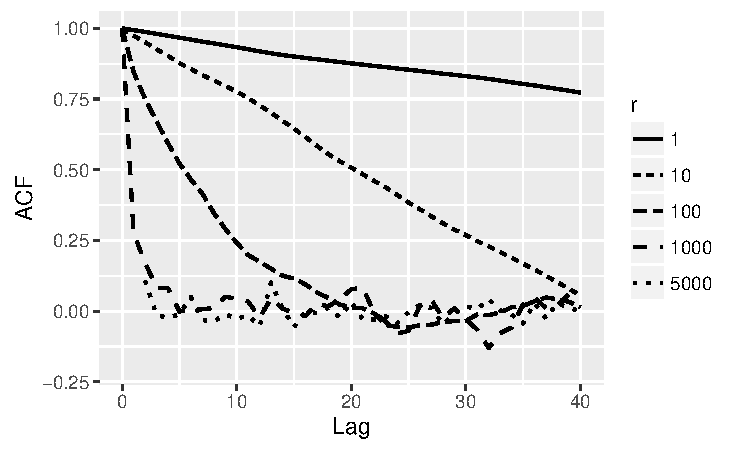
\includegraphics[width=1\textwidth]{probit_demo_acf_prop.pdf}
  \caption{ACF for CDA without M-H adjustment.}
 \label{probit_demo_intercept_proposal}
\end{subfigure}
  \hfill
    \begin{subfigure}[b]{0.32\textwidth}
 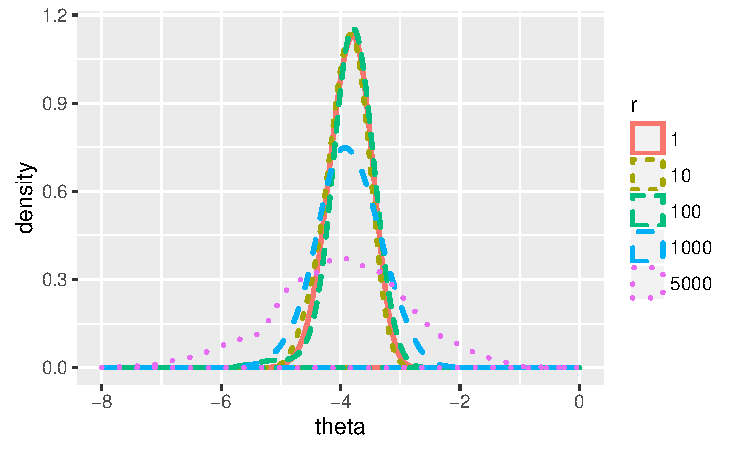
\includegraphics[width=1\textwidth]{density_probit.pdf}
  \caption{Density estimates of the posterior without M-H adjustment.}
   \label{probit_demo_intercept_density}
\end{subfigure}
\hfill
   \begin{subfigure}[b]{0.32\textwidth}
 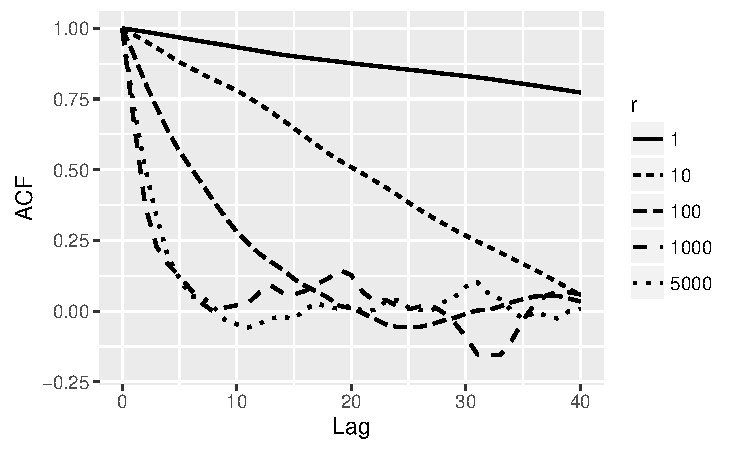
\includegraphics[width=1\textwidth]{probit_demo_acf.pdf}
  \caption{ACF for CDA with M-H adjustment}
   \label{probit_demo_intercept_posteriorsample}
\end{subfigure}
  \hfill
  \caption{ Autocorrelation functions (ACFs) and kernel-smoothed density estimates for different CDA samplers in intercept-only probit model.}
 \label{probit_demo_intercept}
 \end{figure}


\subsection{Choice of calibration parameters} %using Asymptotic Approximation}

As illustrated in the previous subsection, efficiency of CDA is dependent on a good choice of the calibration parameters $r=(r_1,\ldots,r_n)$ and $b=(b_1,\ldots,b_n)$. In the intercept-only case for probit, it was possible to analytically calculate appropriate values of these parameters, but in general an empirical approach is needed. We now propose a simple and efficient algorithm for calculating these parameters relying on Fisher information. In large samples, the Fisher information evaluated at the posterior mode is a good approximation to the posterior covariance. Thus, if we knew the posterior mode under $L_{r,b}$, choosing $r,b$ to minimize
\be
\Delta_{\mc I}(\hat{\theta}_{MAP},\hat{z}_{MAP}) &= \| \mc I_{r,b}(\hat{\theta}_{MAP})-\mc I_{r,b}(\hat{\theta}_{MAP} \mid \hat{z}_{MAP}) \|_F, \\
&=  \left\| \bb E \left[ \left( \frac{\partial}{\partial \theta} \log L_{r,b}(y;\theta) \right)^2 \bigg| \hat{\theta}_{MAP} \right] -  \bb E \left[ \left( \frac{\partial}{\partial \theta} \log f_{r,b}(y;\theta,z) \right)^2 \bigg| \hat{\theta}_{MAP}, \hat{z}_{MAP} \right] \right\|_F
\ee
where $\| A \|_F$ is the Frobenius norm of $A$, would approximate values of $r,b$ that result in fast mixing. 

In general, we do not have access to the posterior mode, so we instead use samples from the Markov chain during an adaptation phase to dynamically update $r_t,b_t$. Specifically, we choose $r_{t+1}$ to minimize $\Delta_{\mc I}(\theta_t,z_t)$, and set $b_{t+1}$ to minimize $|L_{1,0}(\theta_t;y)- L_{r_{t+1},b_{t+1}}(\theta_t;y)|$. Thus, we use $r$ to reduce autocorrelation in the neighborhood of $(\theta_t, z_t)$, and $b$ to make make $L_{r,b}$ close to $L_{1,0}$ in the neighborhood of $\theta_t$. Intuitively, this will make the target distribution closer to the invariant measure of CDA Gibbs, and correspondingly increase the MH acceptance rate. For a concrete illustration, we describe the updating of $r,b$ in the probit case. Putting $\eta_i = x_i\theta$, the Fisher information based on the marginal and the conditional posteriors are:
\be
\mc I_{r,b}(\theta) &= X'\diag\bigg\{\frac{\phi(\eta_i)^2}{ {\Phi(\eta_i)(1- \Phi(\eta_i))}}\bigg\} X,\qquad \mc I_{r,b}(\theta \mid z) = X' R^{-1} X
\ee
respectively, where $\phi$ is the standard normal density. Therefore, setting $r_i = \frac{\Phi(\eta_i)(1- \Phi(\eta_i))} {\phi(\eta_i)^2}$ makes $\Delta_{\mc I}(\theta_t,z_t)=0$.  The $r_i$'s can be calculated using this expression at low cost without calculating the full information matrix. We then choose $b_t$ to increase the acceptance rate in the M-H step, $1\wedge \prod_i \frac{   L_{r,b}(\eta_i;y_i) L(\eta_i^*;y_i)}{ L_{r,b}(\eta_i^*;y_i)L(\eta_i;y_i) }$. As $\eta_i^*$ is unknown before proposed, we set $b_i = \eta_i (\sqrt{r_i}-1)$ to ensure that $L_{r,b}(\eta_i;y_i) = L(\eta_i;y_i)$ and proposals near $\eta_i$ have relatively large acceptance rate.


The proposal kernel we describe above is \emph{adaptive}; that is, we have a collection of proposal kernels $\mc Q = \{Q_{r,b}\}_{(r,b) \in \bb R_+ \times \bb R}$, and we choose a different member of $\mc Q$ at each iteration to create the proposal. The \emph{target} for the resulting transition kernel is $\Pi_{1,0}$ for every $Q_{r,b}$ because of the Metropolis-Hastings rejection step.  In general, ergodicity of adaptive algorithms requires a diminishing adaptation condition; a general condition of this sort is given in (CITE Roberts 2007). Although the algorithm we describe is unlikely to satisfy diminishing adaptation if updating of $r,b$ continues indefinitely, the condition is trivially satisfied by any algorithm that stops adaptation after a fixed number of iterations. Thus, for simplicity, we choose a tuning period length, after which we fix $r,b$ at their current values. More sophisticated adaptation schemes could be devised; however, the fixed tuning period works well empirically.

To illustrate, we consider a probit regression with an intercept and two predictors $x_{i,1},x_{i,2}\sim \No(1,1)$, with $\theta=(-5,1,-1)'$, generating $\sum y_i=20$ among $n=10,000$. The \cite{albert1993bayesian} DA algorithm mixes slowly (Figure~\ref{probit_reg_trace} and \ref{probit_reg_acf}). We also show the 
results of the parameter expansion algorithm (PX-DA) proposed by \cite{liu1999parameter}. PX-DA only mildly reduces the correlation, as it does not solve the variance mismatch problem.  In contrast, applying CDA after a tuning period of 100 iterations, we obtain dramatically better mixing.


 
\begin{figure}[H]
 % \centering
  \begin{subfigure}[b]{0.45\textwidth}
 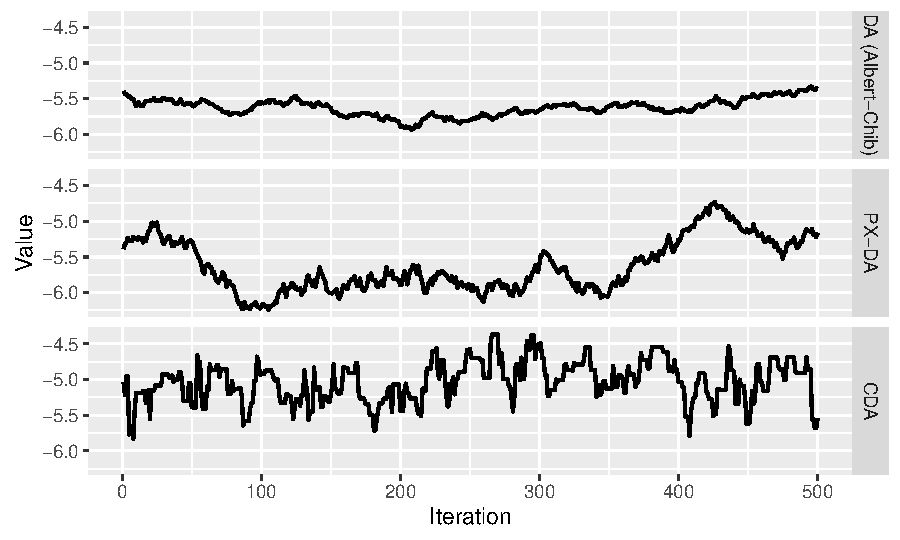
\includegraphics[width=1\textwidth]{probit15_trace_plot.pdf}
  \caption{Traceplot for the original DA, parameter expanded DA and CDA algorithms.}
  \label{probit_reg_trace}
\end{subfigure}
  \hfill
   \begin{subfigure}[b]{0.45\textwidth}
 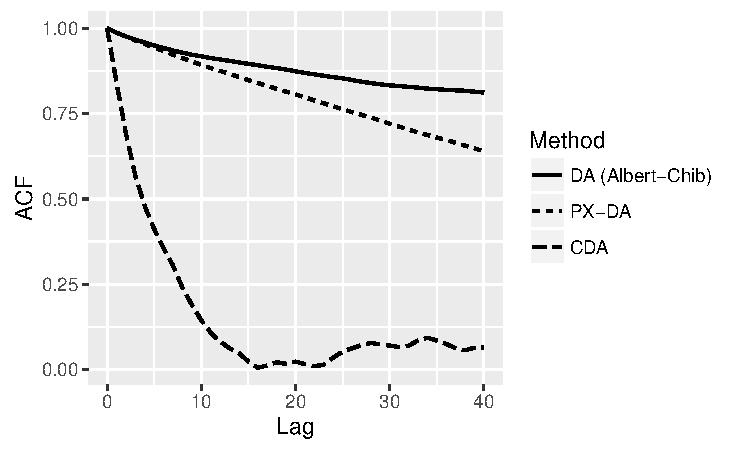
\includegraphics[width=1\textwidth]{probit15_acf.pdf}
  \caption{ACF for original DA, parameter expanded DA and CDA algorithms.}
    \label{probit_reg_acf}
\end{subfigure}
 \caption{Panel (a) demonstrates in traceplot and panel (b) in autocorrelation the substantial improvement in CDA by correcting the variance mis-match in probit regression with rare event data, compared with the original \citep{albert1993bayesian} and parameter-expanded methods \citep{liu1999parameter}.}
 \end{figure}

\subsection{Logistic regression example: A second calibration approach}

Calibration was easy to achieve in the probit examples, because $\mbox{var}( \theta | z,y)$ does not involve the latent variable $z$.  In cases in which the latent variable impacts the variance of the conditional posterior distribution of $\theta$, we propose a different calibration strategy based on inflating the variance of $\pi(z|y)$ targeted towards increasing 
$\bb E_z \mbox{var}(\theta|z,y)$.  In developing this second calibration strategy, we focus on the logistic regression model with 
\be
y_i \sim \Bern(p_i), \quad p_i = \frac{\exp(x_i \theta)}{1+\exp(x_i \theta)},
\ee
and improper prior $\pi(\theta)=1$. For this model, \cite{polson2013bayesian} proposed Polya-Gamma data augmentation:
\be
 z_i &\sim {\PG}(1, |\xtheta|),\\
\theta &\sim \No \left(  (X' Z X)^{-1}   X'  (y-0.5)  ,  (X' Z X)^{-1}  \right),
\ee
where $Z= \diag(z_1,\ldots,z_n)$.  This algorithm relies on expressing the logistic regression likelihood as
$$L(y_i \mid \xtheta)=  \int \exp\{ \xtheta (y_i-1/2)\} \exp\bigg\{ -\frac{z_i (\xtheta)^2}{2}\bigg\} \PG(z_i \mid 1,0) dz_i,$$
where $\mbox{PG}(a_1,a_2)$ denote the Polya-Gamma distribution with parameters $a_1,a_2$, with $\bb{E}z_i= \frac{a_1}{2 a_2}\tanh(\frac{a_2}{2})$.
%As described above, multiplying $r_i$ on $z_i$ is ineffective and makes the integration intractable.

Our previous calibration approach would have relied on inflating the variance in the conditional update of $\theta$, but this unfortunately no longer works well due to the occurence of $Z$ in the conditional covariance.  Instead, we rely on replacing $\PG(z_i \mid 1,0)$ with $\PG(z_i \mid r_i,0)$ in the step for updating the latent data.  Smaller $r_i$ can lead to larger  $\bb E_z \mbox{var}(\theta|z,y)$, providing a route towards calibration.  Applying the bias-adjustment term $b_i$ to the linear predictor $\eta_i = x_i\theta$ leads to 
\be
L_r(\xtheta;y_i) = & \int_{0}^{\infty}  \exp\{ (\xtheta+b_i) (y_i-r_i/2)\} \exp\bigg\{ -\frac{z_i (\xtheta+b_i)^2}{2}\bigg\} \PG(z_i \mid r_i,0) dz_i \\
= &  \frac{\exp \{ (x_i \theta + b_i)y_i \}}{\{1+\exp(\xtheta +b_i)\}^{r_i}},
\label{eq:prop-marginal-logit}
\ee
and the update rule for the proposal:
\be
 z_i &\sim {\PG}(r_i, |\xtheta+b_i|),\\
\theta^* &\sim \No \left(  (X' Z X)^{-1}  X'  (y -r/2- Zb) ,  (X' Z X)^{-1}  \right),
\ee
with acceptance probability:
\be
1 \wedge  \frac{  \prod_i L_r(\xtheta;y_i) L(\xtheta^*;y_i)}{\prod_i  L_r(\xtheta^*;y_i)L(\xtheta;y_i) } =1 \wedge \prod_i  \frac{ \{1+\exp(\xtheta)\}   \{1+\exp(\xtheta^*+b_i)\}^{r_i} } {  \{1+\exp(\xtheta^*)\}  \{1+\exp(\xtheta+b_i)\}^{r_i}    },
\ee
where $L(\theta;y_i)=\frac{\exp(\theta y_i)}{1+\exp(\theta)}$.

To demonstrate why smaller $r_i$ leads to larger $\bb E_z (X' Z X)^{-1}$, we compute the  first negative moment of the Polya-Gamma distribution. Combining \cite{cressie1981moment} and \cite{polson2013bayesian}, $\bb{E}z_i^{-1}= \int_0^{\infty} \prod_{k=1}^{\infty} (1+ d_k^{-1} t) ^{-r_i} dt$ with $d_k=2(k-\frac{1}{2})^2\pi^2 + \frac{(x_i\theta+b_i)^2}{2}$.

For choosing $r$ during tuning, we compare the two Fisher information matrices based on the marginal and conditional; for the latter, we marginalize out $z_i$ by taking the expectation:
\be
X' \diag\bigg\{\frac{\exp(\xtheta)}{ \{1+\exp(\xtheta)\} ^2}\bigg\} X, \quad X'  \diag\bigg\{ \frac{r_i}{2 |\xtheta+b_i|}\tanh\Big(\frac{|\xtheta+b_i|}{2} \Big)\bigg\} X
\ee
To correct the difference, we choose $r_i$ to be $\frac{\exp(\xtheta)}{ \{1+\exp(\xtheta)\} ^2} {2 |\xtheta+b_i|}/ \tanh(\frac{|\xtheta+b_i|}{2})$. To optimize the acceptance rate, given the value of $r_i$ and $\xtheta$,  setting $ \{1+\exp(\xtheta)\}  = \{1+\exp(\xtheta+b_i)\}^{r_i}  $ yields $b_i = \log[  \{1+\exp(\xtheta)\}^{1/r_i} -1] - \xtheta$.


As a numerical illustration, we use a two parameter intercept-slope model with $x_1\sim \No(0,1)$ and $\theta=(-9,1)'$. With $n= 10^5$, we obtain rare outcome data with 
 $\sum y_{i} = 50 $.  We ran the original DA algorithm  \citep{polson2013bayesian} and an independence chain M-H sampler using a multivariate normal proposal $\theta^*|\theta \sim \No(\theta^*| \theta, {\mc I}^{-1}(\theta))$, with ${\mc I}(\theta)$ the Fisher information matrix based on the marginal posterior. For CDA we tuned $r$ and $b$ for $100$ steps, reaching an acceptance rate of $0.8$, and then stopped adaptation and ran an additional burn-in of 100 iterations, with the following 500 samples collected.  Shown in Figure~\ref{logit_random_mixing}, both DA and M-H with a normal proposal mix slowly, exhibiting strong autocorrelation even lag $40$, while CDA has dramatically better mixing.

\begin{figure}[H]
 % \centering
  \begin{subfigure}[b]{0.49\textwidth}
 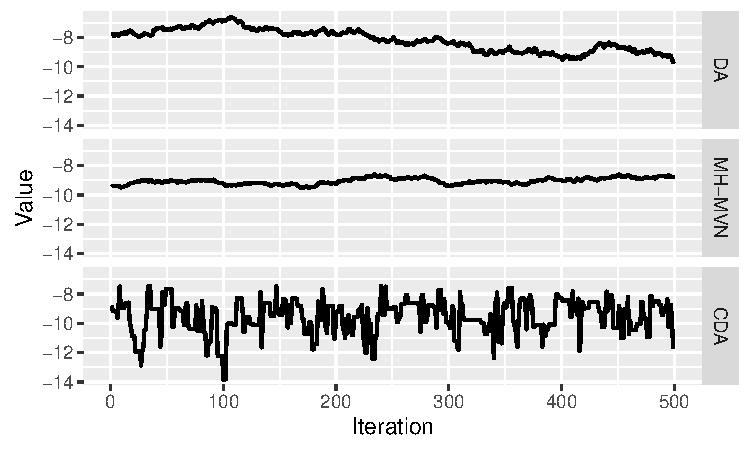
\includegraphics[width=1\textwidth]{logit_demo_trace_plot}
  \caption{Traceplots for DA, CDA and M-H with multivariate normal proposal.}
\end{subfigure}
  \hfill
   \begin{subfigure}[b]{0.49\textwidth}
 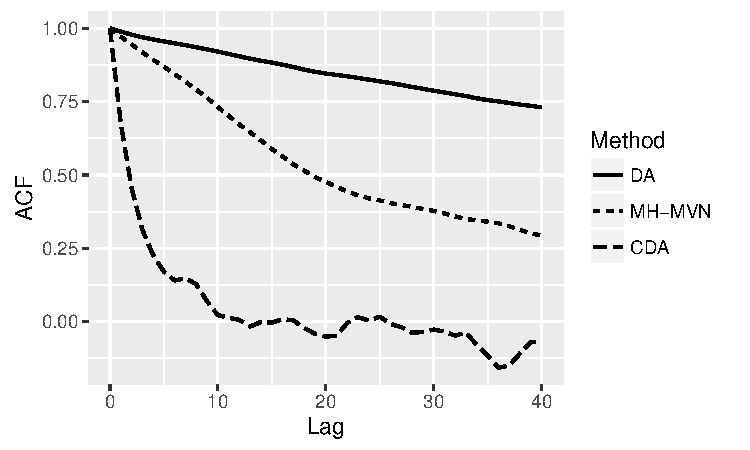
\includegraphics[width=1\textwidth]{logit_demo_acf}
  \caption{ACF for DA, CDA and M-H with multivariate normal proposal.}
\end{subfigure}
 \caption{Panel (a) demonstrates in traceplot and panel (b) in autocorrelation the substantial improvement of CDA in logistic regression with rare event data, compared with the original DA \citep{polson2013bayesian} and the M-H algorithm with multivariate normal proposal (MH-MVN).}
    \label{logit_random_mixing}
 \end{figure}

\James{The section that was previously here seemed mostly duplicative of my edits to earlier parts, so I commented it out} 
 
% \subsection{General Algorithm}
% 
% Before providing theoretical support for CDA, we summarize the algorithm in more generality, noting that substantial further generalizations are possible (e.g., to accommodate hierarchical, temporal and spatial dependence).  We assume the parameters are multi-dimensional and can be divided into two groups $\{ \theta, \tau\}$, with $\theta$ and $\tau$ sampled separately based on their conditional posterior distributions.  For notational ease, we focus on $\theta$ and omit the conditioning on $\tau$ in the rest of the subsection.  Assume $\theta$ can be augmented with latent variable $z$ but is susceptible to slow mixing. The augmented likelihood can be expressed as 
% \be \label{eq:da_decomposition}
% \prod_i L(m_i(\theta);y_i) =\prod_i   \int \pi\left(m_i(\theta)|z_i,y_i \right)\pi(z_i|y_i) d z_i,
% \ee
% where  $m_i(\theta)$ is a continuous and differentiable function $m_i:\bb R^p \mapsto \bb R^d$. For example,  $m_i (\theta) = x_i\theta$ is the linear predictor in regression. Let
% the conditional distribution for $z$ and $\theta$ be, respectively,
% \be
% z_i \mid \theta, y &\sim \pi (z_i; m_i(\theta), y)\\
% \theta \mid z,y &\sim f( \theta; \mu,\Sigma),
% \ee
% where $f( \theta; \mu,\Sigma)\propto \pi(\theta) \prod_i \pi\left(m_i(\theta)|z_i,y_i \right)$. To calibrate the variance $\Sigma$, we introduce a parameter $r_i$. When $\Sigma$ is free from $z$, we put $r_i$ in each $\pi\left(m_i(\theta)|z_i,y_i \right)$ as in the probit examples above. When $\Sigma$ involves $z$, we put $r_i$ in $\pi(z_i|y_i)$ to increase $\bb E_z\Sigma$ as in the logit examples. Then using another parameter $b_i$ to accommodate the shift in $m_i(\theta)$, we obtain the calibrated data augmentation:
% \be \label{eq:cda_decomposition}
% \prod_i L_r(m_i(\theta) ; y_i,  r_i, b_i) = \prod_i \int \pi_r\left(m_i(\theta)+b_i|z_i,y_i \right)\pi_r(z_i|y_i) d z_i.
% \ee
% With prior $\pi(\theta)$, the proposal can then be sampled from the calibrated distribution:
% \be
% z_i & \sim \pi_r(z_i; m_i(\theta)+b_i, y) \\
% \theta^* &\sim f( \theta^*|\mu(r, b),\Sigma(r)).
% \ee
% in an M-H step with acceptance probability:
% \be
% 1 \wedge \prod_i  \frac{L(m_i(\theta^*); y_i) L_r(m_i(\theta) ; y_i)} {L(m_i(\theta); y_i, r_i, b_i) L_r(m_i(\theta^*); y_i, r_i, b_i)}.
% % \label{eq:mh-criterion}
% \ee
% In an initial tuning phase, we adaptively update $r$ and $b$. We choose $r$ at each sampling step to minimize the difference between the Fisher information matrices based on the marginal posterior with the latent data integrated out and the conditional posterior given the latent data.  As illustrated in subsection 2.3-2.4 for the two different strategies of augmentation, simple and computationally efficient closed forms are typically available for the $r_i$'s, which avoid potentially expensive calculation of the full information matrix. Then conditional on $r_i$, we choose $b_i$ to increase the M-H acceptance rate; one choice is the solution to $L_r(m_i(\theta); y_i,  r_i, b_i)=L(m_i(\theta); y_i)$. As a finite approximation for the variance, for some data augmentation, it is possible that Fisher information over estimates the mis-calibration and exhibit low acceptance rate; in that case, we suggest reduce all of the estimated $r_i$'s by a common small fraction to modulate the variance increase to generate higher acceptance rate.



\section{Theory: ergodicity and tuning}
In this section, we provide basic theoretical support for CDA algorithms. First, we show that CDA M-H is ergodic. This is basically a consequence of CDA Gibbs being ergodic for fixed $r,b$ and the fact that $\Pi_{r,b}$ and $\Pi$ are absolutely continuous with respect to Lebesgue measure on $\bb R^p$.
\begin{remark}[ergodicity]
Assume that $\Pi(d\theta)$ and $\Pi_{r,b}(d\theta)$ have densities with respect to Lebesgue measure on $\bb R^p$, and that $K_{r,b}((\theta,z);(\theta',z'))>0 \,\forall\, ((\theta,z),(\theta',z')) \in (\Theta \times \mc Z) \times (\Theta \times \mc Z)$. Then, for fixed $r,b$, CDA Gibbs is ergodic with invariant measure $\Pi_{r,b}(d\theta,dz)$. Moreover, a Metropolis-Hastings algorithm with proposal kernel $Q_{r,b}(\theta';\theta)$ as defined in \eqref{eq:Q} with fixed $r,b$ is ergodic with invariant measure $\Pi(d\theta)$.
\end{remark}
\begin{proof}
For any $r,b$, the conditionals $\Pi_{r,b}(z \mid \theta)$ and $\Pi_{r,b}(\theta \mid z)$ are well-defined for all $z \in \mc Z, \theta \in \Theta$, and therefore the Gibbs transition kernel $K_{r,b}((\theta,z);\cdot)$ and corresponding marginal kernels $Q_{r,b}(\theta;\cdot)$ are well-defined. Moreover, for any $(z,\theta) \in \mc Z \times \Theta$, we have $\bb P[(\theta',z') \in A \mid (\theta,z)] > 0$ by assumption. Thus $K_{r,b}$ is aperiodic and $\Pi_{r,b}$-irreducible.

$Q_{r,b}(\theta';\theta)$ is aperiodic and $\Pi_{r,b}(\theta)$-irreducible, since it is the $\theta$ marginal transition kernel induced by $K_{r,b}((\theta,z);\cdot)$. Thus, it is also $\Pi(\theta)$-irreducible so long as $\Pi \gg \Pi_{r,b}$, where for two measure $\mu,\nu$, $\mu \gg \nu$ indicates absolute continuity. Since $\Pi, \Pi_{r,b}$ have densities with respect to Lebesgue measure, $\Pi_{r,b}$-irreducibility implies $\Pi$ irreducibility. Moreover, $Q(\theta;\theta') > 0$ for all $\theta \in \Theta$. Thus, by Theorem 3 of [CITE Roberts 1994], CDA M-H is $\Pi$-irreducible and aperiodic. 
\end{proof}

%\James{some of the statements above should really become assumptions about CDA gibbs, for example that $\bb P[(\theta',z') \in A \mid (\theta,z)] > 0$ whenever $\Pi_{r,b}(A) > 0$.}

Having established ergodicity of both CDA Gibbs and CDA M-H under weak assumptions that hold for all of the data augmentation strategies we consider here, we now provide a semi-rigorous argument for why our approach to tuning $r$ and $b$ results in both rapid convergence and closeness of $\Pi_{r,b}$ to $\Pi$. Suppose there exists $r$ such that
\be
\bb E_{\Pi_{r,b}}[\var(\theta \mid z)] = \var_{\Pi_{r,b}}(\theta)
\ee
for any value of $b$. This is a simplification, since our adaptation strategies only allow us to control the discrepancy between the Fisher information at the current state.
%for any value of $b$. In general, the  although an analytic expression for the correct value of $r$ may not be available. \James{we should have more justification for this -- is it always true when $r$ is a scale parameter and $b$ a location parameter? What do we need for this to be true?}. 
By tuning $r$ during the adaptation phase to make the lag-1 autocorrelation for the identity function small, we can numerically approximate the correct value of $r$. 

This is obviously much weaker than minimizing the autocorrelation for worst-case functions. However, for the sake of exposition, we will proceed on the assumption that (1) we can make the lag-1 autocorrelation for the identity function zero by appropriately tuning $r$ and (2) this is sufficient to obtain a Gibbs transition kernel that generates nearly \emph{independent} samples. This makes the rationale for tuning $b$ to increase the Metropolis acceptance probability much clearer. First, we note the form of the Metropolis acceptance ratios, which we have used previously without rigorous justification.
\begin{remark}
The CDA M-H acceptance ratio is given by
\be
\frac{L(\theta';y) \Pi^0(\theta') Q_{r,b}(\theta;\theta')}{L(\theta;y) \Pi^0(\theta) Q_{r,b}(\theta';\theta)} = \frac{L(\theta';y)L_{r,b}(\theta;y)}{L(\theta;y) L_{r,b}(\theta';y)} \label{eq:mh-accrat}
\ee
\end{remark}
\begin{proof}
Since $Q_{r,b}(\theta;\theta')$ is the $\theta$ marginal of a Gibbs transition kernel, and Gibbs is reversible on its margins, we have
\be
Q(\theta;\theta') \Pi_{r,b}(\theta) = Q(\theta';\theta) \Pi_{r,b}(\theta),
\ee 
and so
\be
\frac{L(\theta';y) \Pi^0(\theta') Q(\theta;\theta')}{L(\theta;y) \Pi^0(\theta) Q(\theta';\theta)} &= \frac{L(\theta';y) \Pi^0(\theta') L_{r,b}(\theta;y) \Pi^0(\theta) }{L(\theta;y) \Pi^0(\theta) L_{r,b}(\theta';y) \Pi^0(\theta')} \\
&= \frac{L(\theta';y)L_{r,b}(\theta;y)}{L(\theta;y) L_{r,b}(\theta';y)}.
\ee
\end{proof}

The expression in \eqref{eq:mh-accrat} will be near 1 at stationarity if 
\be 
\int \log \left( \frac{L(\theta';y)L_{r,b}(\theta;y)}{L(\theta;y) L_{r,b}(\theta';y)} \right) Q_{r,b}(\theta';\theta) \Pi(d\theta) \approx 0.
\ee
Now, suppose that a Markov chain evolving according to $K_{r,b}$ is rapidly mixing, so that for starting measures satisfying a condition like
\be
\sup_A \frac{\nu(A)}{\Pi_{r,b}(A)} < M
\ee 
for $M$ not too large we have 
\be
\KL{\Pi_{r,b}}{\int Q_{r,b}(\theta';\theta) \nu(d\theta)} \quad \textnormal{small}.
\ee
Then the symmetric KL is 
\be
\KL{\Pi_{r,b}}{\Pi} + \KL{\Pi}{\Pi_{r,b}} &= \int \Pi_{r,b}(d\theta) \log \frac{\Pi_{r,b}(\theta)}{\Pi(\theta)} + \int \Pi(d\theta) \log \frac{\Pi(\theta)}{\Pi_{r,b}(\theta)} \\
&= \int \Pi_{r,b}(d\theta) \log \frac{c_{r,b} L_{r,b}(\theta) \Pi_0(\theta)}{c L(\theta) \Pi_0(\theta)} + \int \Pi(d\theta) \log \frac{c L(\theta) \Pi_0(\theta)}{c_{r,b} L_{r,b}(\theta) \Pi_0(\theta)} \\
&\approx \int K_{r,b}(\theta';\theta) \Pi(d\theta) \log \frac{L_{r,b}(\theta')}{L(\theta')} + \int \Pi(d\theta) \log \frac{L(\theta)}{L_{r,b}(\theta)} \\
&= \bb E \left[ \frac{L_{r,b}(\theta') L(\theta)}{L_{r,b}(\theta) L(\theta')} \right],
\ee
for $\theta \sim \Pi$ and $\theta' \mid \theta \sim K_{r,b}(\theta';\theta)$, so that tuning $b$ to make the M-H acceptance ratio larger will tend to make the symmetric KL between $\Pi_{r,b}$ and $\Pi$ small. This justifies the approach of using the acceptance ratio to tune $b$. As the acceptance ratio approaches 1, CDA M-H and CDA Gibbs coincide, and the CDA Gibbs invariant measure is identically $\Pi$, but the corresponding Gibbs sampler converges rapidly. 

% We studying the theory behind the acceleration of mixing after calibration focusing on samples collected for fixed values of $r,b$ after the adaptation period.
% The mixing rate of a Markov chain can be described by the geometric convergence rate. Let $\mathcal{P}(\theta,.)$ be the Markov transition measure, $\pi(.)$ be the target invariant measure and $\theta$ be the state in the state space $\varTheta$. Starting from the initial state $\theta^{(0)}$, the chain is geometrically ergodic if there exist $M: \varTheta \rightarrow [0, \infty)$ and $\rho\in[0,1)$ such that $||\mathcal{P}^k(\theta,.)-\pi(.) ||_{TV} \le M(\theta^{(0)}) \rho^k$, where $||.||_{TV}$ is the total variation distance $|| P_1 -P_2 ||_{TV} = \underset{\mathcal A\in \mathcal F}\sup ||P_1(\mathcal A)-P_2(\mathcal A)||$. As the number of iterations $k\rightarrow \infty$, $||\mathcal{P}^k(\theta,.)-\pi(.) ||_{TV} \rightarrow 0$ leading to convergence to the target. Slow mixing corresponds to $\rho$ being close to $1$. 
% %As shown by \cite{scott2016bayes}, $\rho$ approaches $1$ as $n$ increases, leading to a complete break-down of algorithm.  {\bf THIS SEEMS THE WRONG CITE AND TOO GENERAL A STATEMENT}
% 
% We first utilize another related quantity, the norm of the forward operator $||\bf{F}||$, which is defined as  ${\bf F}s(\theta)=\int \mathcal{P}(\theta,\theta') s(\theta') d\theta' = E\{ s(\theta') | \theta \}$. In a Hilbert space $L^2(\pi)=\{s(\theta): \bb E s(\theta)=0, \mbox{var}\{s(\theta)\}<\infty \}$, the norm is defined as the maximal correlation between two states $||{\bf F}||=\underset{s(\theta),t(\theta)\in L^2(\pi)}{\sup}\;\mbox{corr}(s(\theta),t(\theta^{'}))$ \citep{liu2008monte}. This norm is related to $\rho$: when the chain is reversible with detailed balance (e.g. M-H), $\lim_{k\rightarrow \infty}||{\bf F}^k||^{1/k}=\rho$; when the chain is non-reversible, $||{\bf F}||^2$ is equal to the convergence rate of the reversibilized chain \citep{fill1991eigenvalue}.
% 
% In each iteration, Gibbs sampling sequentially update all the parameters $\theta$ and the latent variable $z$. We denote the last state as $z'$ and $\theta'$ and the new state as $z$ and $\theta$. Then the original DA sample in the order of $\theta' \rightarrow z' \rightarrow \theta \rightarrow z$, where $a\rightarrow b\rightarrow c$ means that given $b$, $c$ is conditionally independent of $a$.
% 
% In calculation, omitting the first and last steps do not alter the maximal autocorrelation (Lemma 4 in \cite{liu1994collapsed}), leading to:
% 
% \be
% ||{\bf F}_{DA}|| =\underset{s(\theta)\in L^2(\pi)}{\sup}\; \frac{\mbox{var}_{DA} [ \bb E_{DA} \{ s(\theta,z)|\theta^{'},z'\}]}{\mbox{var}_{DA}\{s(\theta,z) \} }  & = \underset{s(\theta)\in L^2(\pi)}{\sup}\; \frac{\mbox{var}_{DA} [ \bb E_{DA} \{ s(\theta)|z'\}]}{\mbox{var}_{DA}\{s(\theta) \} } \\
% & = 1- \underset{s(\theta)\in L^2(\pi)}{\inf}\; \frac{\bb E_{DA}  [  \mbox{var}_{DA}\{ s(\theta)|z'\}]}{\mbox{var}_{DA}\{s(\theta) \} } 
% \label{eq:norm_da}
% \ee
% where the last form without the infimum is known as Bayesian fraction of missing information \citep{papaspiliopoulos2007general}. Slow mixing occurs when ${\bb E_{DA}  [  \mbox{var}_{DA}\{ s(\theta)|z'\}]} \ll {\mbox{var}_{DA}\{s(\theta) \} }$.
% 
% Calibrated DA samples a little differently: by proposing $\theta^*$ in the calibrated sample and using Metropolis-Hastings to accept the new state $\theta^*$ with probability $p(\theta^*,\theta')$ or keep the previous state $\theta$, it in fact samples from a two-component mixture:
% 
% \be
% \theta  \sim (1-p(\theta^*,\theta') ) \delta _{\theta'} + p(\theta^*,\theta') f(\theta^*\mid z').
% \ee
% 
% Therefore, the updating sequence is $\theta'\rightarrow z'$ and $(\theta', z')\rightarrow \theta \rightarrow z$. Similarly, omitting the last step of updating $z$ does not alter the maximal autocorrelation, leading to:
% 
% \be
% ||{\bf F}_{CDA}|| =\underset{s(\theta)\in L^2(\pi)}{\sup}\; \frac{\mbox{var}_{CDA} [ \bb E_{CDA} \{ s(\theta,z)|\theta^{'},z'\}]}{\mbox{var}_{CDA}\{s(\theta,z) \} }  = 1- \underset{s(\theta)\in L^2(\pi)}{\inf}\; \frac{\bb E _{CDA} [  \mbox{var}_{CDA}\{ s(\theta)|z',\theta'\}]}{\mbox{var}_{CDA}\{s(\theta) \} } 
% \label{eq:norm_cda}
% \ee
% 
% 
% To compare the \eqref{eq:norm_da} and \eqref{eq:norm_cda} directly, we rely on the following lemma.
% 
% \begin{lemma}
% 	In Metropolis-Hastings step with current state $\theta'$ and proposal state $\theta^*$ from $f(\theta^*; z')$, if the acceptance probability $p\ge p_0$, the generated state $\theta$ satisfies $\mbox{var}_{CDA}\{ s(\theta)|z', \theta'\} \ge   p_0\cdot \mbox{var}_{CDA} (s(\theta^*)|z')$.
% \end{lemma}
% 
% Therefore, for a given $s(\theta)$, we can induce an increase in $\bb E [\mbox{var}\{ s(\theta')|z'\}]$ by $\gamma$ times over $\bb E [\mbox{var}\{ s(\theta)|z'\}]$, and obtain the following acceleration:
% 
% \begin{theorem}
% Let ${\bf F}_{DA}$ and ${\bf F}_{CDA}$ be the forward operators corresponding to the standard DA and the calibrated DA; $\theta$ be the random variable from the DA updating rule and $\theta^*$ be the one from the CDA proposal. Assume the conditional variance increase in the CDA proposal has ${  \bb E [\mbox {var}_{CDA}\{ s(\theta^*)|z,y\}]  } \ge \gamma \cdot { \bb E [\mbox {var}_{DA}\{ s(\theta)|z,y\}]}$ with the Metropolis-Hastings acceptance probability in \eqref{eq:mh-criterion} greater or equal to $p_0>0$. Then if $p_0 \gamma \ge 1$, 
% $$||{\bf F}_{CDA}||\le 1- \gamma p_0 \cdot \underset{s(\theta)\in L^2(\pi)}{\inf}\; \frac{\bb E_{DA}  [  \mbox{var}_{DA}\{ s(\theta)|z'\}]}{\mbox{var}_{DA}\{s(\theta) \} } 
% \le ||{\bf F}_{DA}||.$$
% \end{theorem}
% 
% It is often not tractable to examine every $s(\theta)\in L^2(\pi)$; but in practice, it suffices to check $s(\theta)=\theta_j$ for every element in $\theta$ \citep{yang2013sequential}. Therefore, the ideal $r_i$ would be close to $\frac{\mbox{var}_{DA}\{\theta \} } {\bb E_{DA}  [  \mbox{var}_{DA}\{ \theta|z'\}]}$ so that $||{\bf F}_{CDA}||\approx 1 - p_0$. Both the numerator and the denominator often lack closed-forms for finite sample, but can be approximately estimated with a term proportional to the Fisher information. As the result, . In our study cases, all of the CDA's have large $p_0$, which is attributed to the distributional similarity between $L_r$ and $L$ in \eqref{eq:mh-criterion}.


\section{Co-Browsing Behavior Application}

We apply CDA to an online browsing activity dataset. The dataset contains a two-way  table of visit count by users who browsed one of $96$ client websites of interests, and one of the  $n=59,792$ high-traffic sites during the same browsing session. We refer to visiting more than one site during the same session as co-browsing. For each of the client websites, it is of large commercial interests find out the high-traffic sites with relatively high co-browsing rates, so that ads can be more effectively placed. For the computational advertising company, it is also useful understand the the co-browsing behavior and predict traffic pattern of users. We consider two models for these data.


\subsection{Hierarchical Binomial Model for Estimating Co-browsing Rates}

We initially focus on one client website and analyze co-browsing rates with the high-traffic sites. With the total visit count $N_i$ available for the $i$th high-traffic site, the count of co-browsing $y_i$ can be considered as the result of a binomial trial. with $y_i$ extremely small relative to $N_i$ (with ratio  ($0.00011 \pm  0.00093$)), the maximum likelihood estimate $y_i/N_i$ can have poor performance. For example, when $y_i=0$, estimating the rate as exactly $0$ is not ideal. Therefore, it is useful to consider a hierarchical model to allow borrowing of information across high-traffic sites.

\be
y_i \sim \Binom\left(N_i, \frac{\exp(\theta_i)}{1+\exp(\theta_i)}\right), \quad \theta_i\stackrel{iid}{\sim} \No(\theta_0, \sigma^2_0), \quad i=1\ldots n\\
(\theta_0,\sigma^2_0) \sim  \pi(\theta_0,\sigma^2_0) 
\ee
Based on expert opinion in quantitative advertising, we use a weakly informative prior $\theta_0\sim \No(-12,49)$ and uniform prior on $\sigma^2_0$. Similar to the logistic regression, we calibrate the binomial Polya-Gamma augmentation, leading to the proposal likelihood:

\be
L_r(\theta_i: y_i,N_i, r_i, b_i) = \frac{\exp(\theta_i+b_i)^y_i}{\{ 1+\exp(\theta_i+b_i)\}^{N_ir_i}}
\ee

Conditioned on the latent Polya-Gamma latent variable $z_i$, each proposal $\theta^*_i$ can be sampled from:

\be
z_i &\sim \PG\left ( (N_ir_i),\theta_i+b_i \right)\\
\theta_i^* &\sim \No \left( \frac{ y_i - r_i N_i/2 -z_i b_i + \theta_0/\sigma^2_0}{z_i+ 1/\sigma^2_0}, \frac{1}{z_i+ 1/\sigma^2_0}\right),
\ee
and accepted or rejected using an M-H step. Similar to logistic regression, the auxiliary parameters are chosen as $r_i =\frac{\exp(\theta_i)}{ \{1+\exp(\theta_i)\} ^2} / \left (   \frac{1}{2 |\theta_i+b_i|} \tanh\frac{|\theta_i+b_i|}{2} \right)$ and $b_i=\log[  \{1+\exp(\theta_i)\}^{1/r_i} -1] - \theta_i$ during adaptation. Since $\theta_i$'s are conditionally independent, the calibrated proposal can be individually accepted with high probability for each $i$. This leads to a high average acceptance of $0.9$, despite the high dimensionality of $59,792$ $\theta_i$'s.

Figure~\ref{data_binomial} shows the boxplots of the ACFs for all $\theta_i$'s. We compare the result with the original DA \citep{polson2013bayesian}. We run DA for $100,000$ steps and CDA for $2,000$ steps, so that they have approximately the same effective sample size. All of the parameters mix poorly in DA; CDA leads to significant improvement with autocorrelation rapidly decaying to close to zero within $5$ lags. Table~\ref{tab:binomial} lists the posterior mean and credible intervals for the parameters, as well as the effective sample size ($T_{eff}$) per iteration, calculated with the \texttt{CODA} package in \texttt{R}.

 To provide a reference, we ran Hamiltonian Monte Carlo (HMC) provided by the \texttt{STAN} software \citep{carpenter2016stan}. HMC enjoys very good mixing performance but is computationally intensive due to the numeric leapfrog steps. The parameter estimates from CDA and HMC are remarkably close, while critically slow mixing in the original DA caused poor estimates.


 \begin{figure}[H]
 % \centering
   \begin{subfigure}[b]{0.32\textwidth}
 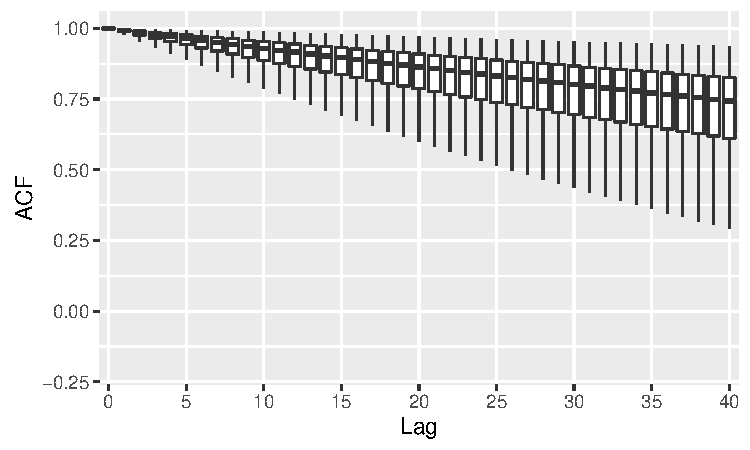
\includegraphics[width=1\textwidth]{binomial_random_acf_da.pdf}
 \caption{ACFs of the rate parameters $\theta_i$ using DA.}
 \end{subfigure}
  \hfill 
 \begin{subfigure}[b]{0.32\textwidth}
 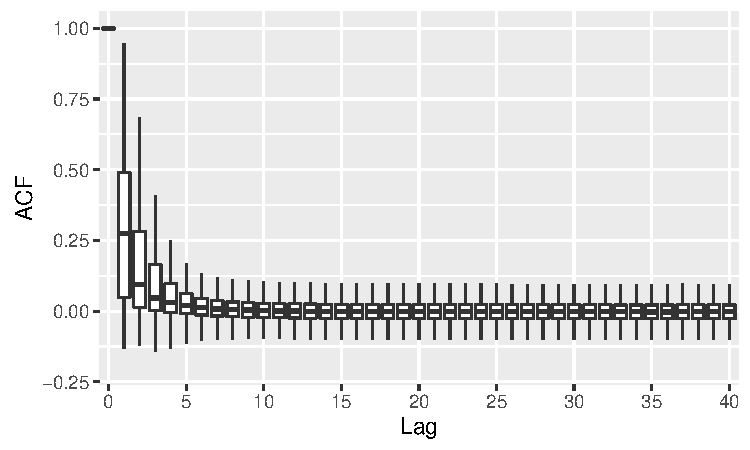
\includegraphics[width=1\textwidth]{binomial_random_acf_cda.pdf}
 \caption{ACFs of the rate parameters $\theta_i$ using CDA.}
 \end{subfigure} 
   \hfill 
 \begin{subfigure}[b]{0.32\textwidth}
 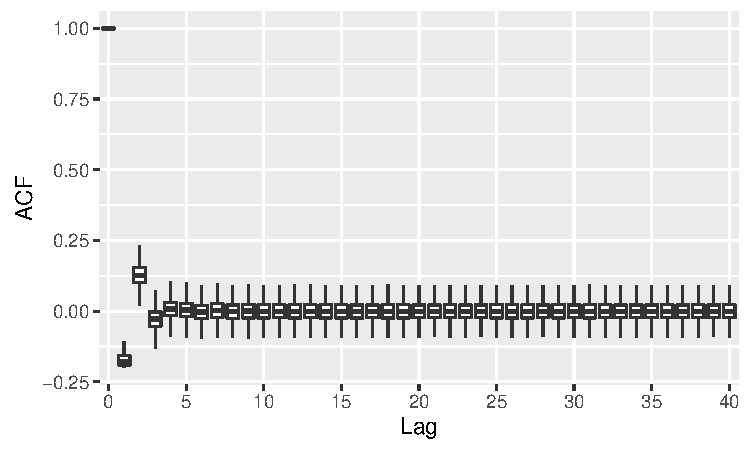
\includegraphics[width=1\textwidth]{binomial_random_acf_hmc.pdf}
 \caption{ACFs of the rate parameters $\theta_i$ using HMC.}
 \end{subfigure} 
 \caption{Boxplots of the ACFs show the mixing of the $59,792$ parameters in the hierarchical binomial model, for the original DA\citep{polson2013bayesian}, CDA and HMC.}
 \label{data_binomial}
 \end{figure}
 
 
 
\begin{table}[H]
\centering
\begin{tabular}{|l |r |r| r| r |} 
 \hline
                          & DA & CDA & HMC\\
 [0.5ex]

 $ \sum \theta_i/n$      & -10.03 (-10.16, -9.87)& -12.05 (-12.09, -12.02) &  -12.06 (-12.09, -12.01)\\
 $ \sum \theta_i^2/n$      & 102.25 (98.92, 105.23)& 153.04 (152.06, 154.05) &  153.17 (152.02, 154.29)\\
$\theta_0$          & -10.03 (-10.17, -9.87)& -12.05 (-12.09,-12.01) &  -12.06 (-12.10, -12.01)\\
$\sigma^2$         & 1.60 (1.36, 1.82)&   7.70 (7.49, 7.88)  & 7.71 (7.51, 7.91)\\
$T_{eff} / T$ & 0.0085 (0.0013 0.0188) & 0.5013 (0.1101,1.0084) & 0.8404 (0.5149, 1.2470)\\
Avg Computing Time /  $T$  & 1.2 sec       & 1.2 sec        & 6 sec\\
Avg Computing Time /  $T_{eff}$  & 140.4 sec       & 0.48 sec        & 1.3 sec\\
 \hline
\end{tabular}
\caption{Parameter estimates (with 95\% credible intervals) and effective sample sizes ($T_{eff}$) of the DA, CDA and HMC in hierarchical binomial model. CDA provides parameter estimates as accurate as HMC, and is more computationally efficient than HMC.}
\label{tab:binomial}
\end{table}


\subsection{Poisson Log-Normal Model for Web Traffic Prediction}

The co-browsing on one high-traffic site and one client site is commonly related to the click-through of user from the former to the latter. Therefore, the count of the co-browsing is a useful indication of the click-through traffic. For any given client website, being able to predict the high traffic sites that could generate most traffic is certainly of high values. Therefore, we consider a Poisson regression model. We choose the co-browsing count of one client website as the outcome $y_i$, and the count of other $95$ websites as the predictor $x^*_{ij}$ for $i=1\ldots 59,792$ and $j=1\ldots 95$. To use them as predictors in Poisson log-normal model, we transform the count onto the log scale with $x_{ij}=\log (x^*_{ij}+1)$. To allow over-dispersion, we use a random intercept for each $i$.


\be
 y_i \sim \Poi \left( \exp  (\xbeta + \tau_i )\right),  \quad \tau_i\stackrel{iid}{\sim} \No(\tau_0, \nu^2), \quad i=1\ldots n\\
 \beta \sim  \No(0, I \sigma_\beta^2), \quad \tau_0 \sim \No(0,\sigma_\tau^2) \quad \nu^2\sim \pi(\nu^2).
\ee
We assign a weakly informative prior for $\beta$ and $\tau_0$ with $ \sigma_\beta^2=\sigma_\tau^2=100$. For the over-dispersion parameter $\nu^2$, we assign a non-informative uniform prior.

To focus on data augmentation, we first rule out other factors that can potentially contribute to slow mixing. In this case,  random effects $\tau_i$ can be problematic for $\beta$ when they are sampled separately. Therefore, we consider sampling $\beta$ and $\tau$ jointly. Using $\tilde X = [ I_n || X ]$ for the $n \times (n+p)$ juxtaposed projection matrix, and $\eta_i=\xbeta + \tau_i$ for the linear predictor, the model can be viewed as a linear predictor with $n+p$ coefficients, for which the parameters $\theta= \{\tau, \beta\}'$ can be sampled jointly in a block. 

The data augmentation for Poisson log-normal model is less known. \cite{zhou2012lognormal} proposed to utilize $\Poi(\eta_i)$ as the limit of the negative binomial $\NB(\lambda,\frac{\eta_i}{\lambda+\eta_i})$ with $\lambda\rightarrow \infty$, and used moderate $\lambda=1,000$ for approximation. The method can be simplified as the following:

\be
L(\xbeta,\tau_i;y)=\frac{1}{ y!}\frac{ \exp(y_i \eta_i \} }{\exp\{\exp(\eta_i)\}} =\frac{1}{ y!} \lim_{\lambda\rightarrow\infty}\frac{\exp(y_i \eta_i)}{\{1+ \exp(\eta_i )/\lambda\}^{\lambda }}.
\label{eq:pos_approx}
\ee

With finite $\lambda$ approximation, it has a Polya-Gamma augmented sampling. Using Gibbs sampler, the approximate posterior can be obtained via:

\be
z_i \sim  \PG ( & \lambda, \eta_i -\log \lambda)\\
\theta \sim  \No (  &  (\tilde X' Z \tilde X+  \begin{bmatrix} 1/\nu^2 \cdot I_n & 0\\ 0 & 1/\sigma^2_{\beta}  \cdot I_p \end{bmatrix})^{-1} \{  \tilde X'  \big ( y - \lambda/2 + Z \log \lambda\big) +   \begin{bmatrix} \tau_0/\sigma^2_{\tau}  1_n \\  0_p \end{bmatrix} \} , \\
& (\tilde X' Z \tilde X+  \begin{bmatrix} 1/\nu^2 \cdot I_n & 0\\ 0 & 1/\sigma^2_{\beta}  \cdot I_p \end{bmatrix})^{-1} ).
\ee

However, this approximate based data augmentation is inherently problematic. For finite $\lambda$ approximation, setting $1,000$ would cause large approximation error. As in \eqref{eq:pos_approx}, the approximating denominator has $(1+\exp\left(\eta_i)/\lambda\right)^\lambda= \exp \{ \exp(\eta_i) + \bigO(\exp(2\eta_i)/\lambda) \}$; for moderately large $\eta_i \approx 10$, $\lambda$ needs to be at least $10^9$ to make $\exp(2\eta_i)/\lambda$ close to $0$. This large error cannot be corrected with an additional M-H step, since the acceptance rate would be too low. On the other hand, it is not practical to use a large $\lambda$  in a Gibbs sampler, since it would otherwise create extremely large $z_i$ and small conditional covariance for $\theta$.

This is where calibration can solve this dilemma. We first choose a very large $\lambda$ ($10^9$) to control the approximation error, then use a small fractional $r_i$ multiplying to $\lambda$ for calibration. This leads to a proposal likelihood similar to the logistic CDA:

\be
L_r(\xtheta;y_i)=\frac{\exp(\eta_i   -\log \lambda +b_i)^{y_i}}{\{1+ \exp(\eta_i -\log \lambda +b_i)\}^{r_i\lambda  }},
\ee
and proposal update rule:

\be
z_i \sim  \PG ( & r_i\lambda, \eta_i -\log \lambda + b_i)\\
\theta^* \sim  \No (  &  (\tilde X' Z \tilde X+  \begin{bmatrix} 1/\nu^2 \cdot I_n & 0\\ 0 & 1/\sigma^2_{\beta}  \cdot I_p \end{bmatrix})^{-1} \{  \tilde X'  \big ( y - r\lambda/2 + Z \log (\lambda -b )\big) +   \begin{bmatrix} \tau_0/\sigma^2_{\tau}  1_n \\  0_p \end{bmatrix} \} , \\
& (\tilde X' Z \tilde X+  \begin{bmatrix} 1/\nu^2 \cdot I_n & 0\\ 0 & 1/\sigma^2_{\beta}  \cdot I_p \end{bmatrix})^{-1} )
\ee

Let $\eta_i^* = \tilde X \theta^*$, the proposal is accepted with probability ( based on Poisson density and the approximation $L_r(\xtheta;y_i)$):
\be
1 \wedge \prod_i  \frac{ \exp \{ \exp (\eta_i)\}}{ \exp \{ \exp (\eta_i^*)\}} \frac {{\{1+ \exp(\eta_i^{*}  -\log \lambda +b_i)\}^{r_i\lambda }}}{{\{1+ \exp(\eta_i  -\log \lambda +b_i)\}^{r_i\lambda  }}}.
\ee
 
During the adaptation, we set $r_i = 1/c_0 \tau_i\exp(\eta_i) /  \left( \frac{\lambda } {2|\eta_i + b_i - \log\lambda|}  \tanh\frac{ |\eta_i + b_i - \log\lambda|}{2} \right )$ based on the Fisher information. We found the acceptance rate too low with $c_0 =1$, which indicates an overestimation of mis-calibration. Therefore, we reduce $c_0$ and obtained an acceptance rate of $0.6$. Conditionally on $r_i$, we used $b_i=\log[ \exp \{ \exp(\eta_i - \log\lambda -\log r_i)   \}-1] -\eta_i + \log\lambda$.


To compare, we ran approximate DA Gibbs sampler with $\lambda=1,000$, CDA with M-H proposal and HMC. We ran approximate DA for $200,000$ steps, CDA for $2,000$ steps and HMC for $20,000$ steps so that they have approximately the same effective sample size. For CDA, we used the first $1,000$ steps for adapting $r$ and $b$. Figure~\ref{data_poisson} shows the mixings of DA and CDA. Surprisingly, even with small $\lambda$, in approximate DA, all of the parameters still mix poorly; HMC seemed to be impacted by the random effects and most of parameters remain highly correlated within $40$ lags; CDA substantially improves the mixing. Table~\ref{table:Poisson} compares all three algorithms. CDA is clearly the best algorithm to generate the highest effective sample size within the same computing time.


 \begin{figure}[H]
 % \centering
  \begin{subfigure}[b]{0.32\textwidth}
 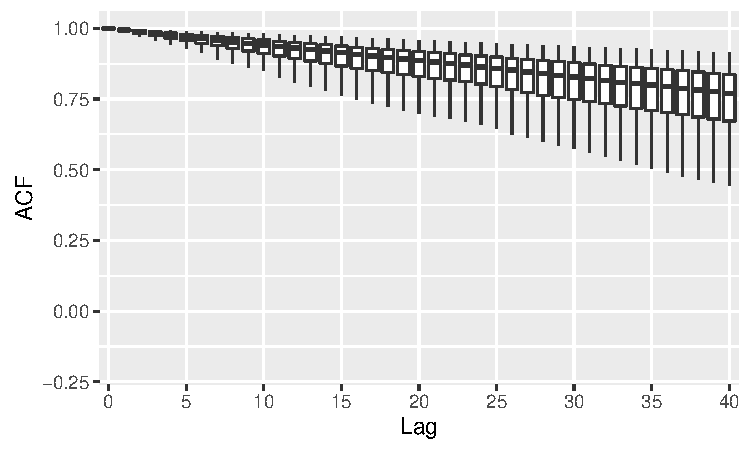
\includegraphics[width=1\textwidth]{poisson_acf_da}
 \caption{Autocorrelation of the parameters from DA.}
 \end{subfigure}
  \hfill 
 \begin{subfigure}[b]{0.32\textwidth}
 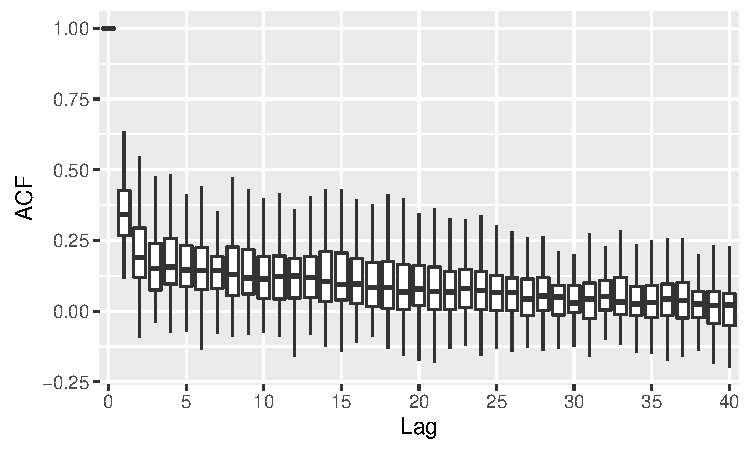
\includegraphics[width=1\textwidth]{poisson_acf_cda}
 \caption{Autocorrelation of the parameters from CDA.}
 \end{subfigure}  \hfill 
 \begin{subfigure}[b]{0.32\textwidth}
 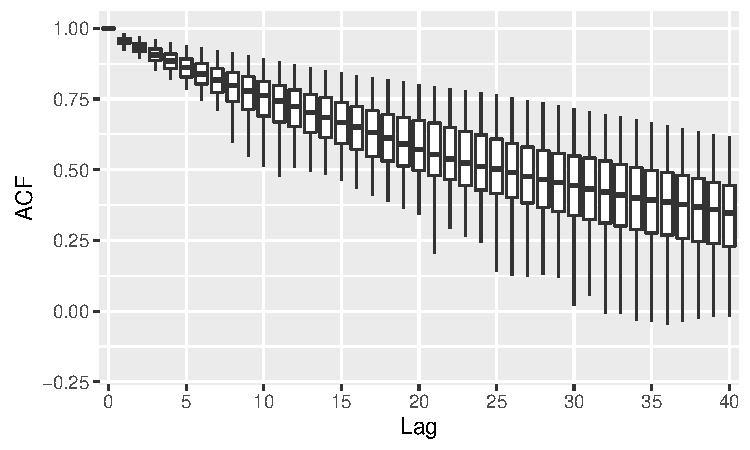
\includegraphics[width=1\textwidth]{poisson_acf_hmc}
 \caption{Autocorrelation of the parameters from HMC.}
 \end{subfigure}
 \caption{CDA significantly improves the mixing of the parameters in the Poisson log-normal.}
 \label{data_poisson}
 \end{figure}



To evaluate the prediction performance, we use another dataset $\{y_{i,new},x_{i,new} \}$ collected during a different time period for validation. We use the posterior mean $\{\hat\tau, \hat \beta\}$ for the prediction $\hat y_{i,new}=\exp( x_{i,new}{\hat\theta} + \hat\tau_i)$; cross-validation root-mean-squared error between $y_{i,new}$ and $\hat y_{i,new}$ is computed. CDA performs quite well and the validation error that is $4$ times lower than DA.


\begin{table}[H]
\centering
\begin{tabular}{|l |r |r| r| r |} 
 \hline
                          & DA & CDA & HMC\\
 [0.5ex]
$\sum \beta_j / 95$         & 0.072 (0.071, 0.075)&  -0.041 (-0.042, -0.038)  & -0.010 (-0.042, -0.037) \\
$\sum \beta_j^2 / 95$         & 0.0034 (0.0033, 0.0035)&  0.231 (0.219 0.244)  & 0.232 (0.216 0.244)   \\
$\sum\tau_i/n$         & -0.405 (-0.642, -0.155)&  -1.292 (-2.351, -0.446)  &  -1.297 (-2.354, -0.451)  \\
$\sum\tau_i^2/n$         & 1.126 (0.968, 1.339)&  3.608 (0.696, 7.928)  & 3.589 (0.678, 8.011)  \\
% RMSE                              & 30.83        & 4.03          & 7.38\\
Prediction RMSE                           & 33.21        & 8.52          & 13.18\\
$T_{eff} / T$ & 0.0037 (0.0011 0.0096) & 0.3348 (0.0279, 0.699) &  0.0173 (0.0065, 0.0655) \\
Avg Computing Time /  $T$  & 1.3 sec       & 1.3 sec        & 56 sec\\
Avg Computing Time /  $T_{eff}$  & 346.4 sec       & 11.5 sec        & 3240.6 sec\\
 \hline
\end{tabular}
\caption{Parameter estimates, prediction error and computing speed of the DA, CDA and HMC in Poisson regression model.}
\label{table:Poisson}
\end{table}

\section{Discussion}
Data augmentation is a useful technique to sample posterior from the closed-form conditional. It has been discovered that it could severely slow down the mixing, caused by the gap between conditional variance given augmented data and marginal variance. With data size increases and become complex, it is common for the conditional distribution of the parameter to deviate from the area that has reasonable mixing performance. As we show in the previous examples, this quickly leads to an un-manageable increase in the computational time and poor performance in estimation.

To address this problem, we propose a general class of method to calibrate the conditional variance. With a new parameter to adjust the step size, the transition in each iteration is increased onto the same order of the marginal variance. The generated samples are used as proposal in the Metropolis-Hastings to obtain correct posterior. In this article, we demonstrate that this strategy is generally applicable when $\theta \mid z$ belongs to the location-scale family. We expect it to be extensible to any conditional distribution with a variance or scale.

We would like to draw some further comparison between CDA and HMC. Both algorithms rely on finding good proposal by searching an area far from the current state. The key difference lies in the computing efficiency. HMC is computationally intensive since Hamiltonian dynamics often requires multiple numeric steps, as it lacks closed-form solution in most of time. CDA adds a little extra cost to the original Gibbs sampler and needs only one step for generating proposal. Therefore, when the data augmentation exists, CDA is always much more efficient.

In this article, we insist on obtaining the exact posterior, to provide an analysis on the mixing property. Without the Metropolis-Hastings step, the sampling strategy in calibrated data augmentation can be used alone to generate approximate posterior.

\bibliography{reference}
\bibliographystyle{plainnat}


\section{Appendix}

%
%\subsubsection{Proof of Theorem 1:}
%
%
%Let $\theta=\{\theta_1, \theta_2\}$ be the parameters that are divided into two parts. Let $\theta'$ and $z'$ be the parameters and latent variables in the last iteration. Omitting $y$ for the ease of notation, the square of maximal correlation can be represented as $||{\bf F}||^2=\underset{s(\theta,z),t(\theta,z)\in L^2(\pi)}{\sup}\;\mbox{corr}\{s(\theta,z),t(\theta^{'},z')\}^2
%= \underset{s(\theta,z)\in L^2(\pi)}{\sup}\; \frac{\mbox{var} [ E \{ s(\theta,z)|\theta^{'},z'\}]}{\mbox{var}\{s(\theta,z) \} }$.
%
%The original DA samples in the order of $ \{\theta'_1, \theta'_2\} \rightarrow z' \rightarrow \{\theta_1, \theta_2\}\rightarrow z$, with $ \mbox{var} [ E \{ s(\theta,z)|\theta^{'},z'\}] =  \mbox{var} [ E \{ s(\theta_1, \theta_2,z)|\theta^{'}_1,\theta^{'}_2,z'\}] $. The marginalization and sampling based CDA samples  in the order of $ \theta'_2 \rightarrow z' \rightarrow \theta_2\rightarrow z$, followed by $z' \rightarrow \theta'_1$ and  $z \rightarrow \theta_1$ with $ \mbox{var} [ E \{ s(\theta,z)|\theta^{'},z'\}] =  \mbox{var} [ E \{ s(\theta_1, \theta_2,z)|\theta^{'}_1,\theta^{'}_2,z'\}] = \mbox{var} [ E \{ s(\theta_1, \theta_2,z)|\theta^{'}_2,z'\}]$.
%
%For better clarity, let $E_{X}$ denote the integration over $P(dX)$. 
%
%\begin{equation}
%\begin{aligned}
% \mbox{var} [ E \{ s(\theta_1, \theta_2,z)|\theta^{'}_2,z'\}]  & = E_{\theta^{'}_2,z'}  [ E_{\theta_1, \theta_2,z}\{ s(\theta_1, \theta_2,z)|\theta^{'}_2,z' \} ]^2 -  (E_{\theta^{'}_2,z'}   [ E_{\theta_1, \theta_2,z}\{ s(\theta_1, \theta_2,z)|\theta^{'}_2,z' \} ])^2  \\
% & = E_{\theta^{'}_2,z'}   [ E_{\theta'_1}E_{\theta_1, \theta_2,z} \{ s(\theta_1, \theta_2,z)|\theta'_1, \theta^{'}_2,z' \} ]^2 - (E_{\theta^{'}_1,\theta^{'}_2,z'}   [ E_{\theta_1, \theta_2,z} \{ s(\theta_1, \theta_2,z)|\theta^{'}_1,\theta^{'}_2,z' \} ])^2 \\
%& \le  E_{\theta^{'}_2,z'}  E_{\theta'_1} [ E_{\theta_1, \theta_2,z} \{ s(\theta_1, \theta_2,z)|\theta'_1, \theta^{'}_2,z' \} ]^2 - (E_{\theta^{'}_1,\theta^{'}_2,z'}   [ E_{\theta_1, \theta_2,z} \{ s(\theta_1, \theta_2,z)|\theta^{'}_1,\theta^{'}_2,z' \} ])^2\\
%& =  \mbox{var}  [E \{ s(\theta_1, \theta_2,z)|\theta^{'}_1,\theta^{'}_2,z'\}] 
%\end{aligned}
%\end{equation}
%
%This completes the proof.


\subsection{Proofs}

\subsubsection{Lemma 1}
As the M-H step in CDA is equivalent to sampling from the mixture that:

\be
(1-p)\delta_{\theta'} + p f_{CDA}(\theta^*; z')
\ee
where $p$ is the acceptance probability in \eqref{eq:mh-criterion} and $f_{CDA}$ is the calibrated proposal distribution. Its conditional variance is:

\be
  \mbox{var}_{CDA}\{ s(\theta)|z', \theta'\} = & (1-p) s(\theta')^2 + p \bb E_{CDA} \{ s(\theta^*)^2|z'\}  - [ (1-p) s(\theta') + p \bb E_{CDA} \{ s(\theta^*)|z'\}]^2 \\
  = & (1-p) [s(\theta')^2 - (1-p) s(\theta')^2 - 2p s(\theta')  \bb E_{CDA} \{ s(\theta^*)|z'\}  + p \bb E_f \{ s(\theta^*)|z'\}^2 ] \\
  & + p [\bb E_{CDA} \{ s(\theta^*)^2|z'\} - \bb E_{CDA} \{ s(\theta^*)|z'\}^2]\\
  = & (1-p)p [s(\theta') - \bb E_{CDA} \{ s(\theta^*)|z'\}]^2 + p \cdot \mbox{var}_{CDA} (s(\theta^*)|z') \\
  \ge &  p\cdot \mbox{var}_{CDA} (s(\theta^*)|z') \\
  \ge &  p_0\cdot \mbox{var}_{CDA} (s(\theta^*)|z')
\ee



\subsubsection{Theorem 1}

With Lemma 1,
\be
\bb E [  \mbox{var}_{CDA}\{ s(\theta)|z', \theta'\} ]  
\ge &  p_0 \bb \cdot \bb E [\mbox{var}_{CDA} (s(\theta^*)|z') ]\\
\ge &  p_0 \gamma  \cdot \bb E [\mbox{var}_{DA} (s(\theta^*)|z')].
\ee

Since the marginal variances are the same for two algorithms $\mbox{var}_{DA}\{s(\theta) \} = \mbox{var}_{CDA}\{s(\theta) \}$. When $p_0\gamma \ge 1$, rearranging terms and taking supremum on both sides complete the proof.

%
%\subsubsection{Proof of Theorem 3:}
%
%Without loss of generality, take $M\ge 1$, then $E |\theta_j| {1}_{|\theta_j|>M}\le E \theta_j^2 {1}_{|\theta_j|>M}\le \epsilon_2$.
%
%\begin{equation}
%\begin{aligned}
%|E (\theta_j |y)-E_{r,b} (\theta_j |y)| & = \int  | \theta_j \pi(\theta_j | y) -  \theta_j\pi_{r,b}(\theta_j|y)| d\theta_j  \\
%& \le \int  | \theta_j| |\pi(\theta_j | y) - \pi_{r,b}(\theta_j|y)| d\theta_j  \\
%& =   \int  1(|\theta_j|\le M) | \theta_j|\cdot |\pi(\theta_j | y) - \pi_{r,b}(\theta_j|y)| d\theta_j  +  \int 1(|\theta_j|>M) | \theta_j| |\pi(\theta_j | y) - \pi_{r,b}(\theta_j|y)| d\theta_j  \\
%& \le M   \int   |\pi(\theta_j | y) - \pi_{r,b}(\theta_j|y)| d\theta_j  + \int 1(|\theta_j|>M) | \theta_j| \pi(\theta_j | y) d\theta_j +  \int 1(|\theta_j|>M) | \theta_j| \pi_{r,b}(\theta_j|y) d\theta_j  \\
%& \le 2M\epsilon_1 + 2\epsilon_2 \\
%& = 2M\epsilon_1 + o(\epsilon_1),
%\end{aligned}
%\end{equation}
%where triangle inequality and the definition of total variation distance are used.
%
%
%
%\begin{equation}
%\begin{aligned}
%|\mbox{var} (\theta_j |y)-\mbox{var}_{r,b} (\theta_j |y)| & = | [E (\theta^2_j |y)- \{ E(\theta_j |y)\}^2] - [ E_{r,b} (\theta^2_j |y)-\{ E_{r,b} (\theta_j |y)\}^2 ]|\\
%& \le | E (\theta^2_j |y)-  [ E_{r,b} (\theta^2_j |y) ] |+ | \{ E(\theta_j |y)\}^2 -\{ E_{r,b} (\theta_j |y)\}^2 ]|\\
%& \le 2M^2 \epsilon_1 + 2\epsilon_2 + | \{ E(\theta_j |y)\} -\{ E_{r,b} (\theta_j |y)\} ]| \cdot | \{ E(\theta_j |y)\}+\{ E_{r,b} (\theta_j |y)\}]| \\
%& \le 2M^2 \epsilon_1 + 2\epsilon_2 +  (2M\epsilon_1 + 2\epsilon_2) \{  2 E(\theta_j |y) + 2M\epsilon_1 + 2\epsilon_2 \} \\
%& \le 2M^2 \epsilon_1 + 2\epsilon_2 +  (2M\epsilon_1 + 2\epsilon_2) \{  2 M+ 2\epsilon_2 + 2M\epsilon_1 + 2\epsilon_2 \} \\
%& = 6M^2\epsilon_1 + o(\epsilon_1).
%\end{aligned}
%\end{equation}
%
%
%To prove Corollary 1, using Cauchy-Schwarz inequality $ \{  E\theta_{j_1}\theta_{j_2} 1(\theta_{j_1}>M_{j_1} )  1(\theta_{j_2}>M_{j_2} )    \}^2 \le   E\theta^2_{j_1}1(\theta_{j_1}>M_{j_1} )  E \theta^2_{j_2} 1(\theta_{j_1}>M_{j_2} )   =\epsilon^2_2$. Following the similar proof for variance, it can be derived that:
%
%$$|\mbox{cov}(\theta_{j_1},\theta_{j_2}|y)-\mbox{cov}_{r,b}(\theta_{j_1},\theta_{j_2}|y)|\le 6M_{j_1}M_{j_2}\epsilon_1+o(\epsilon_1 ).$$
%
%\subsubsection{Proof of Theorem 4:}
%
%Since $\theta= B^{-} B\theta$, $\mbox{cov} B\theta= B^{-}  \mbox{cov} B\theta B^{-T} $, applying H\"older's inequality:
%
%$$||{E}\theta-{E}\theta_{r,b}||_1 \le ||B^{-}||_1 ||{E}B\theta- {E}B\theta_{r,b}||_\infty$$
%$$||\mbox{cov}\theta-\mbox{cov}\theta_{r,b}||_1 \le  ||B^{-}||_\infty ||B^{-}\mbox{cov} B\theta- B^{-}\mbox{cov}B\theta_{r,b}||_1 \le ||B^{-}||_1 ||B^{-}||_\infty ||\mbox{cov} B\theta- \mbox{cov}B\theta_{r,b}||_\infty$$
%
%\subsection{Approximation Error in Logistic Regression}
%
%For better clarity, we renumber the double index $ij$ using single index $i$.
%
%\subsubsection{Total Variation Distance}
%
%The individual Kullback-Leibler distance:
%
%\begin{equation}
%\begin{aligned}
%KL\{ { L_{r,b}(y_i|\eta_{i}) } || {L(y_i|\eta_{i})} \}& =\mbox{E}\log \frac{\Gamma(1/r_i+1) r_i^{y_i}  /\Gamma(1/r_i -y_i+1)  }{\Gamma(2) /\Gamma(2 -y_i)  } + \log \frac{ 1+\exp(\eta_{i})}{ \{1+\exp(\eta_{i})r_i\}^{1/r_i}}\\
%& =\log\{1+ \exp ( \eta_{i})\}   - 1/r \log\{1+ r\exp ( \eta_{i})\}\\
%& \le   \{   (r_i-1) \frac{ \exp(2\eta_{i})}{2} \}  1\{\exp(\eta_{i})< 1/r_i\} + \log \frac{ 1+\exp(\eta_{i})}{ \{1+\exp(\eta_{i})r_i\}^{1/r_i}}  1\{\exp(\eta_{i})\ge 1/r_i\} \\
%%& \le   \frac{r_i-1}{2 r_i^2}  1\{r_i <\exp(-\eta_{i}) \} + \log \frac{ 1+\exp(\eta_{i})}{ \{1+\exp(\eta_{i})r_i\}^{1/r_i}}  1\{ \eta_{i} \ge -\log r_i\}.
%\label{KL_logit}
%\end{aligned}
%\end{equation}
%
%
%With adaptive $r_i=1$ if $\eta_{i}\ge -\log r_i$ and Pinsker's inequality,
%
%$$||P_{r,b}(y_i|\eta_{i}) - P(y_i|\eta_{i})||_{TV} \le   \{   \frac{\sqrt{r_{i}-1}  \exp(\eta_{i})}{2} \} 1 \{\eta_{i}< - \log r_{i} \le 0 \}$$
%
%\subsubsection{Tail Integral}
%
%Consider each likelihood $L(y_i|p_i) = p^y_i (1-p)^{1-y_i}$ with $p_i=\frac{\exp(\eta_{i})}{1+\exp(\eta_{i})}$. Applying density transformation leads to 
%$\pi(\eta_{i}|y_i) = \frac{\exp(\eta_{i}) \exp(y_i\eta_{i})}{\{1+\exp(\eta_{i})\}^3}$.
%
%If $y_i=1$,
%\begin{equation}
%	\begin{aligned}
%			\mbox{E}\{ \eta_{i}^2 1(|\eta_{i}|>M) \} & = E\{ \eta_{i}^2 1(|\eta_{i}|>M, \eta_{i} \ge 0 ) \} + E\{ \eta_{i}^2 1(|\eta_{i}|>M, \eta_{i}<0 ) \} \\
%	& \le \int_M^{\infty} \frac{\eta_{i}^2}{1+\exp(\eta_{i})} d\eta_{i} + \int_{-\infty}^{-M}{\eta_{i}^2}{\exp(2\eta_{i})}d\eta_{i}  \\
%	& \le \int_M^{\infty} {\eta_{i}^2}{\exp(-\eta_{i})} d\eta_{i} +\int_{-\infty}^{-M}{\eta_{i}^2}{\exp(2\eta_{i})}d\eta_{i} \\
%	& = (M^2+2M+2)\exp(-M) + \frac{1}{4} (2M^2 + 2M +1) \exp(-2M).
%	\end{aligned}
%\end{equation}
%
%if $y_i=0$,
%\begin{equation}
%	\begin{aligned}
%			\mbox{E}\{ \eta_{i}^2 1(|\eta_{i}|>M) \} & = \mbox{E}\{ \eta_{i}^2 1(|\eta_{i}|>M, \eta_{i} \ge 0 ) \} + E\{ \eta_{i}^2 1(|\eta_{i}|>M, \eta_{i}<0 ) \} \\
%	& \le \int_M^{\infty} \frac{\eta_{i}^2}{\{1+\exp(\eta_{i})\}^2} d\eta_{i} + \int_{-\infty}^{-M}{\eta_{i}^2}{\exp(\eta_{i})}d\eta_{i}  \\
%	& \le \int_M^{\infty} {\eta_{i}^2}{\exp(-2\eta_{i})} d\eta_{i} + \int_{-\infty}^{-M}{\eta_{i}^2}{\exp(\eta_{i})}d\eta_{i} \\
%	& =\frac{1}{4} (2M^2 + 2M +1) \exp(-2M)+  (M^2+2M+2)\exp(-M) .
%	\end{aligned}
%\end{equation}
%
%Therefore, the tail square integral is in $O(M^2 \exp(-M))$.
%
%
%Consider the approximate density $L_{r,b} (y_i| \eta_i) =\frac{\Gamma(1/r_i+1)}{\Gamma(1/r_i-y_i+1)\Gamma(y_i+1)} p^{y_i} (1-p)^{(1/r_i-y_i)}$, where $p=\frac{\exp ( \eta_i+\log r_i)}{\{1+ \exp ( \eta_i +\log r_i)\}}$ and $y_i< 1/r_i+1$.  Applying density transformation leads to $\pi(\eta_{i}|y_i) = \frac{\Gamma(1/r_i+1)}{\Gamma(1/r_i-y_i+1)\Gamma(y_i+1)}\frac{\{r_i\exp(\eta_{i})\}^{(y_i+1)}}{\{1+r_i\exp(\eta_{i})\}^{(1/r_i+2)}}$.
%
%\begin{equation}
%	\begin{aligned}
%			\mbox{E}_{r,b}\{ \eta_{i}^2 1(|\eta_{i}|>M) \}  % = \mbox{E}_{r,b}\{ \eta_{i}^2 1(|\eta_{i}|>M, \eta_{i} \ge 0 ) \} + \mbox{E}_{r,b}\{ \eta_{i}^2 1(|\eta_{i}|>M, \eta_{i}<0 ) \} \\
%	&	 \le      \int      \eta_i^2  1(|\eta_{i}|>M)  \frac{\Gamma(1/r_i+1)r_i^{y_i}}{\Gamma(1/r_i-y_i+1)}\frac{r_i}{\Gamma(y_i+1)}\frac{\{\exp(\eta_{i})\}^{(y_i+1)}}{\{1+r_i\exp(\eta_{i})\}^{(1/r_i+2)}} d\eta_i  \\
%	&  \le \int \eta_i^2  1(|\eta_{i}|>M) \frac{r_i}{y_i!}\frac{\{\exp(\eta_{i})\}^{(y_i+1)}}{\{1+r_i\exp(\eta_{i})\}^{(1/r_i+2)}} d\eta_i  \\	
%		& \le \frac{1}{y_i! r_i^{y_i}} \int_M^{\infty} \frac{\eta_{i}^2}{1+r_i\exp(\eta_{i})} d\eta_{i} +  \frac{r_i}{y_i!} \int_{-\infty}^{-M}{\eta_{i}^2}{\exp\{\eta_{i} (y_i+1) \}}d\eta_{i} \\
%		& \le \frac{1}{y_i! r_i^{y_i+1}} \int_M^{\infty} {\eta_{i}^2}{\exp(-\eta_{i})} d\eta_{i} +  \frac{r_i}{y_i!} \int_{-\infty}^{-M}{\eta_{i}^2}{\exp\{\eta_{i} (y_i+1) \}}d\eta_{i} \\
%	& = \frac{1}{y_i! r_i^{y_i+1}} (M^2+2M+2)\exp(-M) + \frac{r_i}{y_i!}   (M^2+2M+2)\exp(-M) 
%	\end{aligned}
%\end{equation}
%
%\subsection{Approximation Error in Poisson Log-Linear Model}
%
%\subsubsection{Total Variation Distance}
%
%With $\eta_i=\xtheta$, the individual Kullback-Leibler distance:
%
%\begin{equation}
%\begin{aligned}
%KL\{ { L_{r,b}(y_i|\eta_{i}) } || {L(y_i|\eta_{i})} \}& =\mbox{E}\log \frac{\Gamma(1/r_i+1) r_i^{y_i}  }{\Gamma(1/r_i -y_i+1)   } + \log \frac{ \exp\exp(\eta_{i})}{ \{1+\exp(\eta_{i})r_i\}^{1/r_i}}\\
%& \le \exp ( \eta_{i})   - 1/r \log\{1+ r\exp ( \eta_{i})\}\\
%& \le   \{   r_i \frac{ \exp(2\eta_{i})}{2} \}  1\{\exp(\eta_{i})< 1/r_i\} + \log \frac{ \exp\exp(\eta_{i})}{ \{1+\exp(\eta_{i})r_i\}^{1/r_i}} 1\{\exp(\eta_{i})\ge 1/r_i\} \\
%\label{KL_poisson}
%\end{aligned}
%\end{equation}
%
%With adaptive $r_i = 0$ if $\eta_{i}\ge 1/r_i$ and Pinsker's inequality,
%$$||P_{r,b}(y_i|\eta_{i}) - P(y_i|\eta_{i})||_{TV} \le   \{   \frac{\sqrt{r_{i}}  \exp(\eta_{i})}{2} \} 1 \{\eta_{i}< - \log r_{i} \}$$
%
%
%
%\subsubsection{Tail Integral}
%
%
%Consider each likelihood $L(y_i|p_i) = {p_i^{y_i}\exp(-p_i)}/{y_i!}$ with $p_i={\exp(\eta_{i})}$. Applying density transformation leads to 
%$\pi(\eta_{i}|y_i) = \exp \{\eta_i (y_i+1)\} \exp\{-\exp(\eta_i) \} /{y_i!}$. Without loss of generality, assume $|M|\ge 1$.
%
%
%\begin{equation}
%	\begin{aligned}
%			E\{ \eta_{i}^2 1(|\eta_{i}|>M) \} & = E\{ \eta_{i}^2 1(|\eta_{i}|>M, \eta_{i} \ge 0 ) \} + E\{ \eta_{i}^2 1(|\eta_{i}|>M, \eta_{i}<0 ) \} \\
%	& \le \int_M^{\infty}  \frac{ \exp \{\eta_i (y_i+3)\}  \} }{\exp\{\exp(\eta_i)\} e^2 y_i!} d\eta_{i} + \int_{-\infty}^{-M}  \frac {\eta_{i}^2 \exp \{ \eta_{i} (y_i+1)\}  }{ y_i !}d\eta_{i}  \\
%	& =  \frac{IGamma(y_i+3, \exp(M)\} }{e^2 y_i!} +   \frac{IGamma(3, (y_i+1)M)\} }{(y_i+1)^3 y_i!} .
%	\end{aligned}
%\end{equation}
%where $IGamma(a,b)$ is the incomplete Gamma function $\int_b^{\infty} t^{a-1} \exp(-t) dt$, equal to the $\{1-F(b) \} \Gamma(a)$, with $F(b)$ as the cumulative distribution function of gamma distribution ${\mathcal G}(a,1)$.
%
%
%Similar to the logistic approximate, consider the approximate density $L_{r,b} (y_i| \eta_i) =\frac{\Gamma(1/r_i+1)}{\Gamma(1/r_i-y_i+1)\Gamma(y_i+1)} p^{y_i} (1-p)^{(1/r_i-y_i)}$, where $p=\frac{\exp ( \eta_i+\log r_i)}{\{1+ \exp ( \eta_i +\log r_i)\}}$ and $y_i< 1/r_i+1$.  Applying density transformation leads to $\pi(\eta_{i}|y_i) = \frac{\Gamma(1/r_i+1)}{\Gamma(1/r_i-y_i+1)\Gamma(y_i+1)}\frac{\{r_i\exp(\eta_{i})\}^{(y_i+1)}}{\{1+r_i\exp(\eta_{i})\}^{(1/r_i+2)}}$.
%
%
%Note when $\eta_i>0$ hence $r_i < 1/exp(0)=1$, $\frac{1}{1+r_i\exp(\eta_{i})\}^{(1/r_i)}}\le \frac{1}{1+ \exp(\eta_{i})} $. Then,
%
%\begin{equation}
%	\begin{aligned}
%			\mbox{E}_{r,b}\{ \eta_{i}^2 1(|\eta_{i}|>M) \}  % = \mbox{E}_{r,b}\{ \eta_{i}^2 1(|\eta_{i}|>M, \eta_{i} \ge 0 ) \} + \mbox{E}_{r,b}\{ \eta_{i}^2 1(|\eta_{i}|>M, \eta_{i}<0 ) \} \\
%	&	 \le      \int      \eta_i^2  1(|\eta_{i}|>M)  \frac{\Gamma(1/r_i+1)r_i^{y_i}}{\Gamma(1/r_i-y_i+1)}\frac{r_i}{\Gamma(y_i+1)}\frac{\{\exp(\eta_{i})\}^{(y_i+1)}}{\{1+r_i\exp(\eta_{i})\}^{(1/r_i+2)}} d\eta_i  \\
%	&  \le \int \eta_i^2  1(|\eta_{i}|>M) \frac{r_i}{y_i!}\frac{\{\exp(\eta_{i})\}^{(y_i+1)}}{\{1+r_i\exp(\eta_{i})\}^{(1/r_i+2)}} d\eta_i  \\	
%		& \le \int_M^{\infty} \frac{r_i}{y_i! r_i^{y_i+1}}\frac{\eta_i^2}{\{1+r_i\exp(\eta_{i})\}} d\eta_i 
%				+  \frac{r_i}{y_i!} \int_{-\infty}^{-M}{\eta_{i}^2}{\exp\{\eta_{i} (y_i+1) \}}d\eta_{i} \\
%	& =  \frac{1}{y_i! r_i^{(y_i+1)}}   (M^2+2M+2)\exp(-M) + \frac{r_i}{y_i!}    \frac{IGamma(3, (y_i+1)M)\} }{(y_i+1)^3 }
%	\end{aligned}
%\end{equation}





\subsection{Goodness-of-Fit and Cross-Validation for Poisson Regression}


 \begin{figure}[H]
 % \centering
   \begin{subfigure}[b]{0.45\textwidth}
 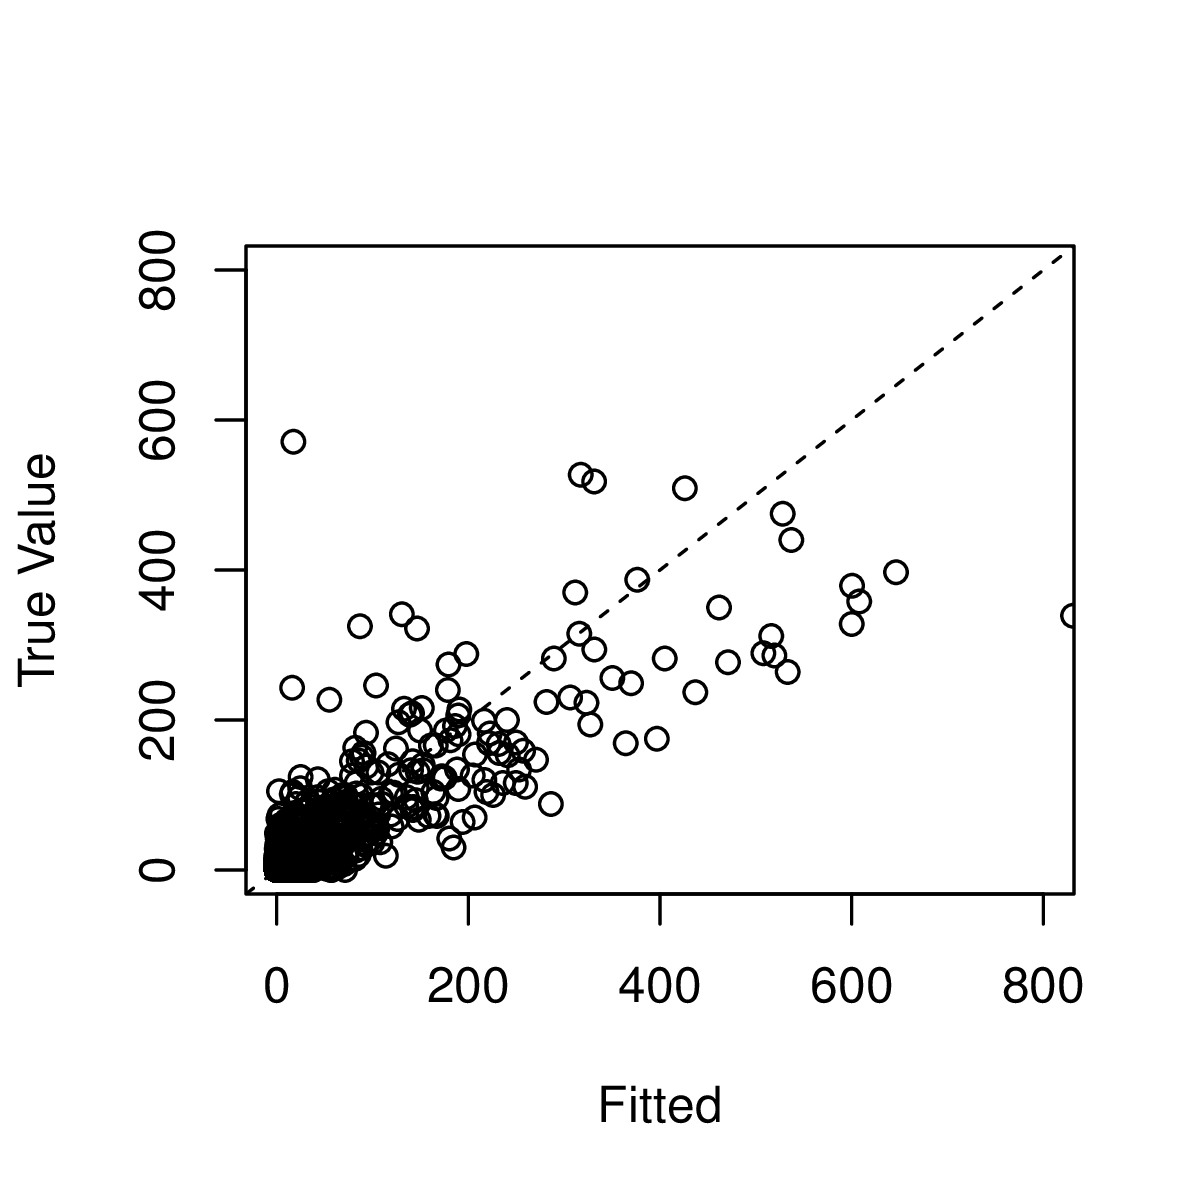
\includegraphics[width=1\textwidth]{poisson_fitting_da.png}
 \caption{Fitted vs true values using DA}
 \end{subfigure}
  \hfill 
 \begin{subfigure}[b]{0.45\textwidth}
 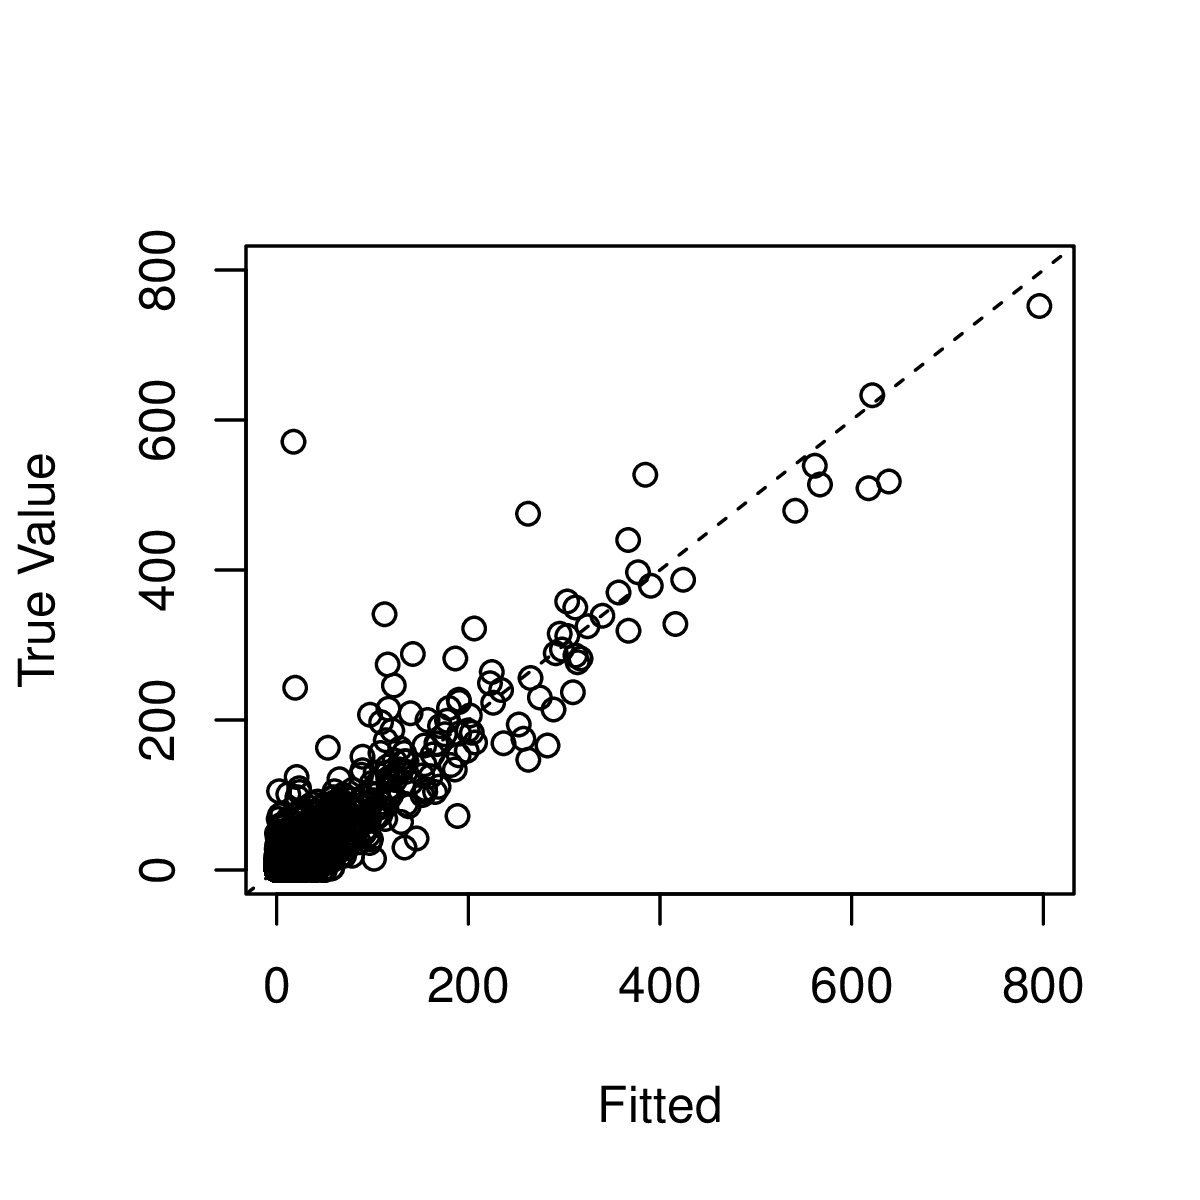
\includegraphics[width=1\textwidth]{poisson_fitting_ada.png}
 \caption{Fitted vs true values using CDA}
 \end{subfigure}  
   \begin{subfigure}[b]{0.45\textwidth}
 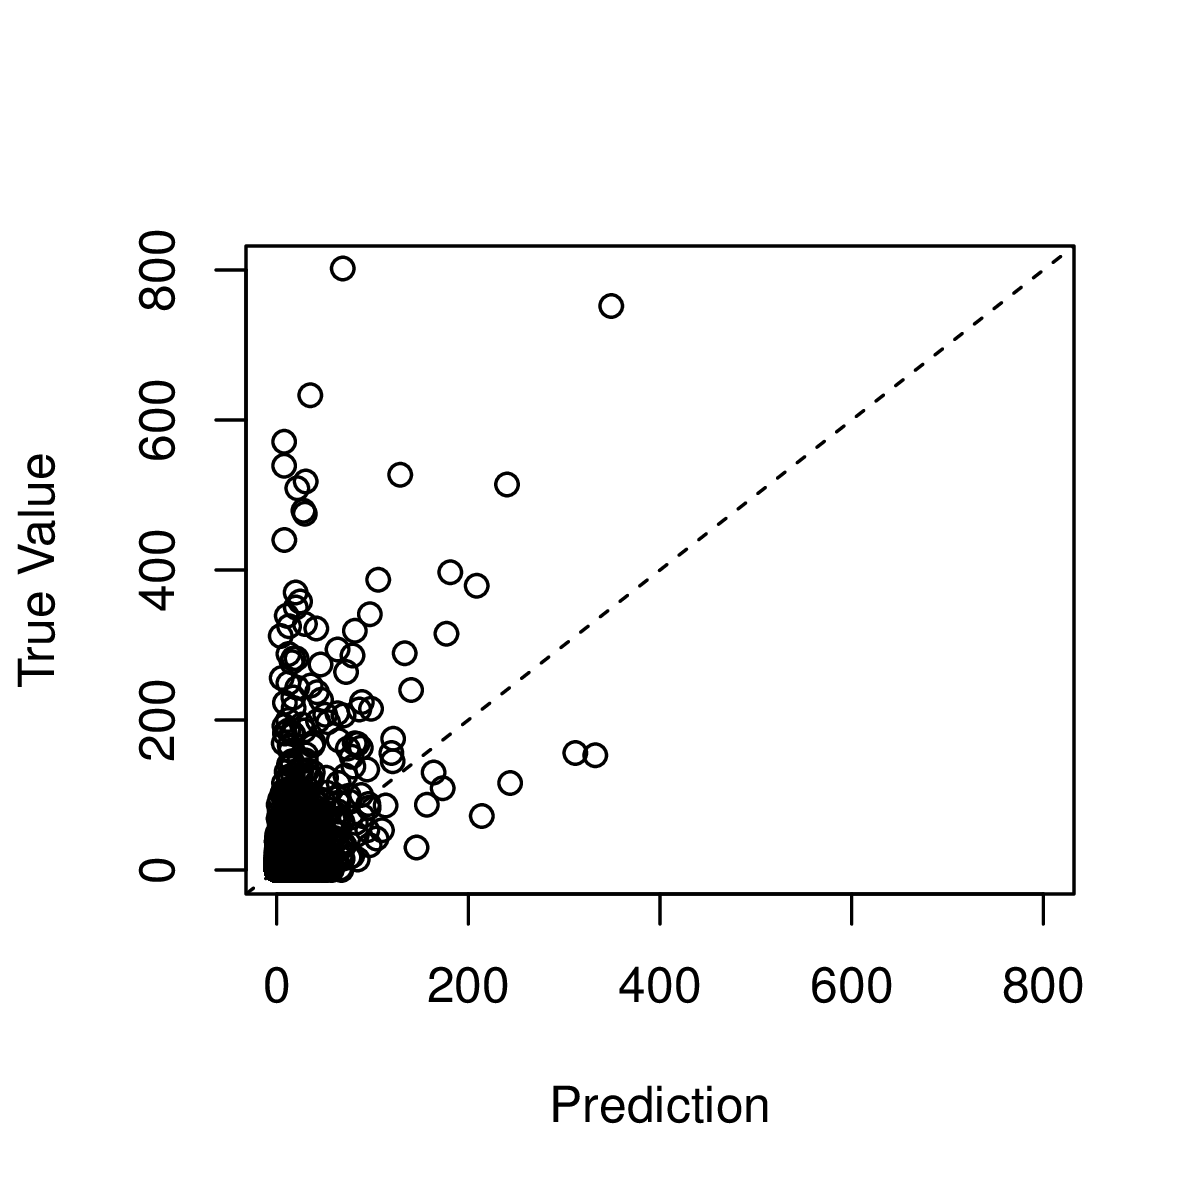
\includegraphics[width=1\textwidth]{poisson_cv_da.png}
 \caption{Prediction vs true values using DA}
 \end{subfigure}
  \hfill 
 \begin{subfigure}[b]{0.45\textwidth}
 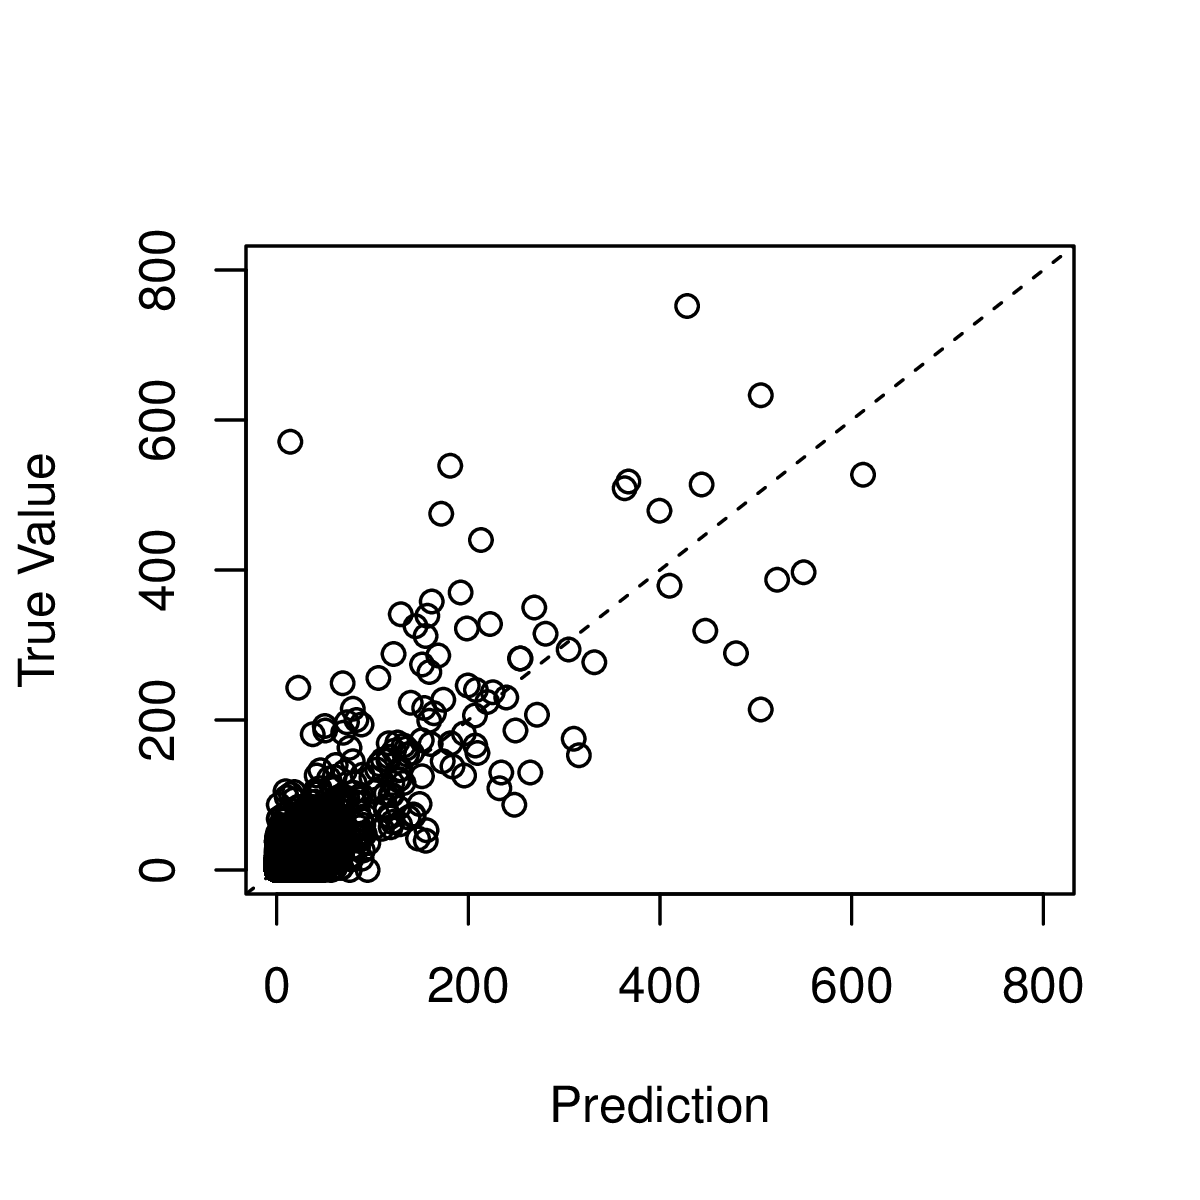
\includegraphics[width=1\textwidth]{poisson_cv_ada.png}
 \caption{Prediction vs true values using CDA}
 \end{subfigure} 
 \caption{The posterior estimates produced by CDA is better fitted to the data and have more accurate prediction than DA.}
 \end{figure}

 % \subsection{Comparing posterior samples of CDA with HMC}
% \begin{figure}[H]
%  % \centering
%    \begin{subfigure}[b]{0.45\textwidth}
%  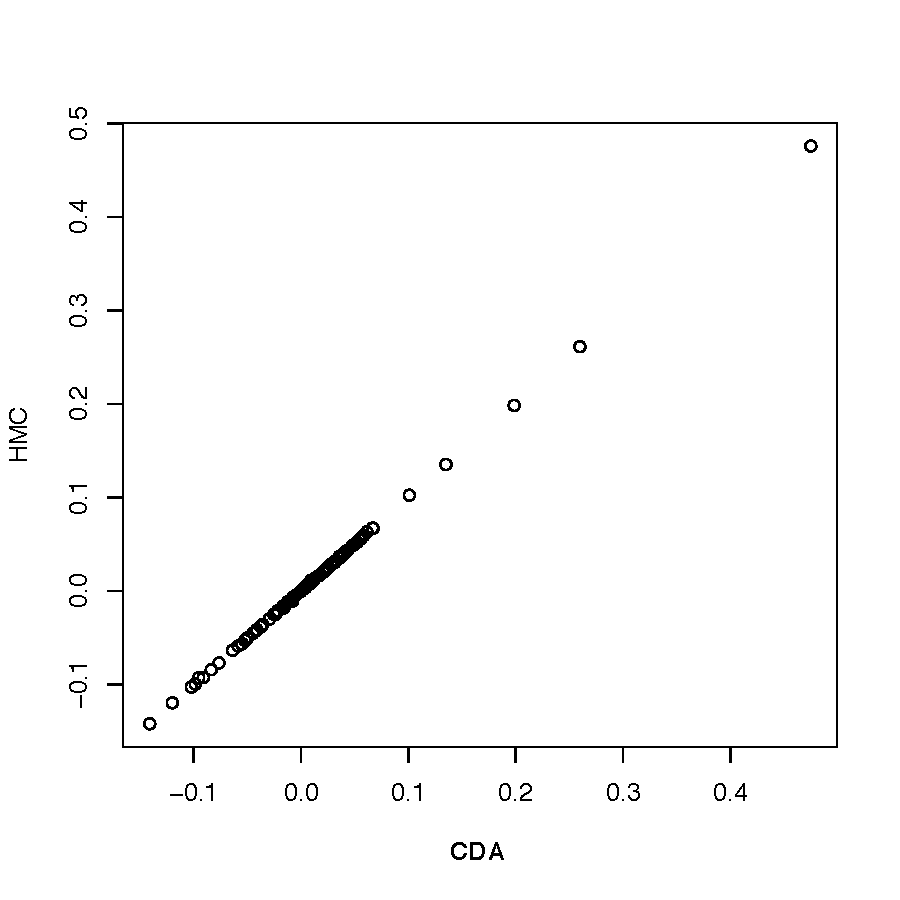
\includegraphics[width=1\textwidth]{CDAvsHMC_mean.pdf}
%  \caption{Comparing posterior means for $\theta_1,\dots \theta_{95}$ from the HMC and CDA. The  RMSE between the two is $0.0007$.}
%  \end{subfigure}
%   \hfill 
%  \begin{subfigure}[b]{0.45\textwidth}
%  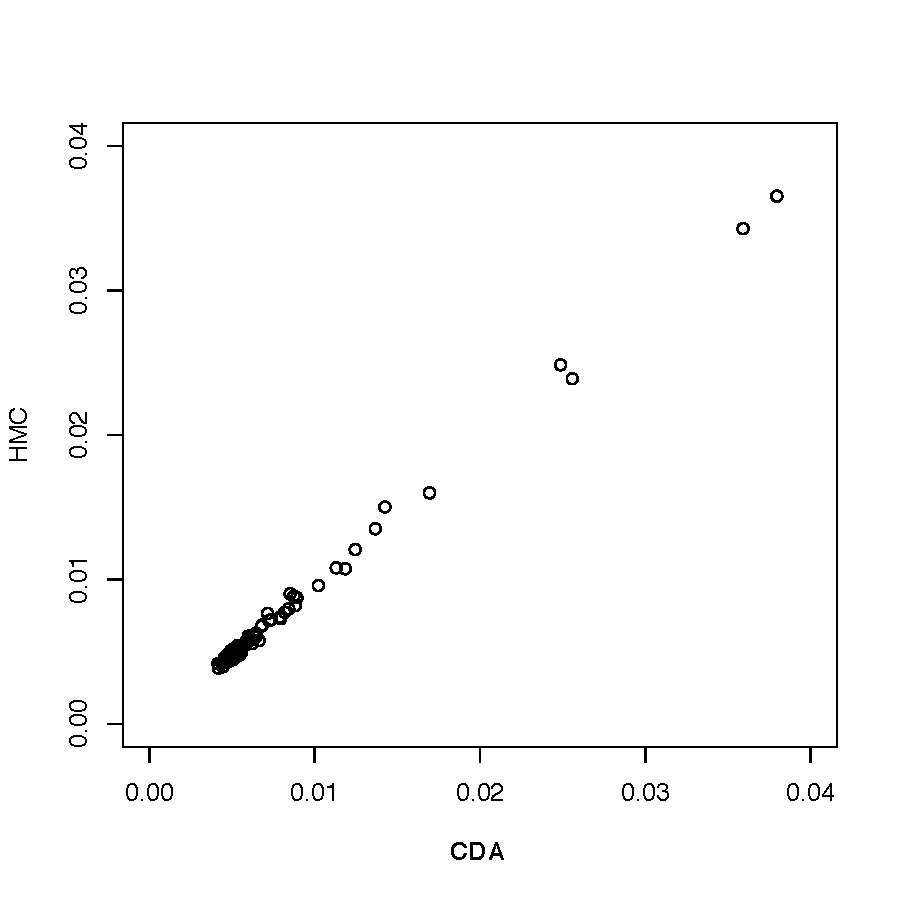
\includegraphics[width=1\textwidth]{CDAvsHMC_sd.pdf}
%  \caption{Comparing posterior standard deviation for $\theta_1,\dots \theta_{95}$ from the HMC and CDA.  The  RMSE between the two is $0.0004$.}
%  \end{subfigure}  
%  \caption{The results from CDA and HMC agree very well.}
%  \end{figure}





 
\end{document}




